%% abtex2-modelo-trabalho-academico.tex, v-1.9.2 laurocesar
%% Copyright 2012-2014 by abnTeX2 group at http://abntex2.googlecode.com/ 
%%
%% This work may be distributed and/or modified under the
%% conditions of the LaTeX Project Public License, either version 1.3
%% of this license or (at your option) any later version.
%% The latest version of this license is in
%%   http://www.latex-project.org/lppl.txt
%% and version 1.3 or later is part of all distributions of LaTeX
%% version 2005/12/01 or later.
%%
%% This work has the LPPL maintenance status `maintained'.
%% 
%% The Current Maintainer of this work is the abnTeX2 team, led
%% by Lauro César Araujo. Further information are available on 
%% http://abntex2.googlecode.com/
%%
%% This work consists of the files abntex2-modelo-trabalho-academico.tex,
%% abntex2-modelo-include-comandos and abntex2-modelo-references.bib
%%

% ------------------------------------------------------------------------
% ------------------------------------------------------------------------
% abnTeX2: Modelo de Trabalho Academico (tese de doutorado, dissertacao de
% mestrado e trabalhos monograficos em geral) em conformidade com 
% ABNT NBR 14724:2011: Informacao e documentacao - Trabalhos academicos -
% Apresentacao
% ------------------------------------------------------------------------
% ------------------------------------------------------------------------

\documentclass[
	% -- opções da classe memoir --
	12pt,				% tamanho da fonte
	openright,			% capítulos começam em pág ímpar (insere página vazia caso preciso)
	twoside,			% para impressão em verso e anverso. Oposto a oneside 
	% oneside twoside twoside openright openany onecolumn twocolumn
	a4paper,			% tamanho do papel. 
	% -- opções da classe abntex2 --
	%chapter=TITLE,		% títulos de capítulos convertidos em letras maiúsculas
	%section=TITLE,		% títulos de seções convertidos em letras maiúsculas
	%subsection=TITLE,	% títulos de subseções convertidos em letras maiúsculas
	%subsubsection=TITLE,% títulos de subsubseções convertidos em letras maiúsculas
	% -- opções do pacote babel --
	english,			% idioma adicional para hifenização
	french,				% idioma adicional para hifenização
	spanish,			% idioma adicional para hifenização
	brazil				% o último idioma é o principal do documento
	]{abntex2}

% ---
% Pacotes básicos 
% ---
\usepackage{lmodern}			% Usa a fonte Latin Modern			
\usepackage[T1]{fontenc}		% Selecao de codigos de fonte.
\usepackage[utf8]{inputenc}		% Codificacao do documento (conversão automática dos acentos)
\usepackage{lastpage}			% Usado pela Ficha catalográfica
\usepackage{indentfirst}		% Indenta o primeiro parágrafo de cada seção.
\usepackage{color}				% Controle das cores
\usepackage{graphicx}			% Inclusão de gráficos
\usepackage{microtype} 			% para melhorias de justificação
\usepackage{array}
% ---

%força tabelas a nao reposicionarem		
\usepackage{placeins}

%adiciona pdfs ao documento
\usepackage{pdfpages}

%citação usando modelo autor - data

% apendice
%\usepackage[titletoc]{appendix}
%\renewcommand\cftappendixname{\appendixname~}
%\AtBeginDocument{\renewcommand\appendixname{New Name}}

%%%CODE
\usepackage{listings}
\usepackage{caption}

\lstset{literate=
  {á}{{\'a~}}1 {é}{{\'e~}}1 {í}{{\'i~}}1 {ó}{{\'o~}}1 {ú}{{\'u~}}1
  {ã}{{\~a~}}1 {ẽ}{{\~e~}}1 {ĩ}{{\~i~}}1 {õ}{{\~o~}}1 {ũ}{{\~u~}}1
  {Á}{{\'A~}}1 {É}{{\'E~}}1 {Í}{{\'I~}}1 {Ó}{{\'O~}}1 {Ú}{{\'U~}}1
  {à}{{\`a~}}1 {è}{{\`e~}}1 {ì}{{\`i~}}1 {ò}{{\`o~}}1 {ù}{{\`u~}}1
  {À}{{\`A~}}1 {È}{{\'E~}}1 {Ì}{{\`I~}}1 {Ò}{{\`O~}}1 {Ù}{{\`U~}}1
  {ä}{{\"a~}}1 {ë}{{\"e~}}1 {ï}{{\"i~}}1 {ö}{{\"o~}}1 {ü}{{\"u~}}1
  {Ä}{{\"A~}}1 {Ë}{{\"E~}}1 {Ï}{{\"I~}}1 {Ö}{{\"O~}}1 {Ü}{{\"U~}}1
  {â}{{\^a~}}1 {ê}{{\^e~}}1 {î}{{\^i~}}1 {ô}{{\^o~}}1 {û}{{\^u~}}1
  {Â}{{\^A~}}1 {Ê}{{\^E~}}1 {Î}{{\^I~}}1 {Ô}{{\^O~}}1 {Û}{{\^U~}}1
  {œ}{{\oe~}}1 {Œ}{{\OE~}}1 {æ}{{\ae~}}1 {Æ}{{\AE~}}1 {ß}{{\ss~}}1
  {ç}{{\c c~}}1 {Ç}{{\c C~}}1 {ø}{{\o~}}1 {å}{{\r a~}}1 {Å}{{\r A~}}1
  {€}{{\EUR~}}1 {£}{{\pounds~}}1
}



\definecolor{dkgreen}{rgb}{0,0.6,0}
\definecolor{gray}{rgb}{0.5,0.5,0.5}
\definecolor{mauve}{rgb}{0.58,0,0.82}

\lstset{frame=tb,
  language=bash,
  aboveskip=3mm,
  belowskip=3mm,
  showstringspaces=false,
  columns=flexible,
  basicstyle={\small\ttfamily},
  numbers=none,
  numberstyle=\tiny\color{gray},
  keywordstyle=\color{blue},
  commentstyle=\color{dkgreen},
  stringstyle=\color{mauve},
  breaklines=true,
  breakatwhitespace=true,    % added this
  tabsize=3
}
%\DeclareCaptionFormat{listing}{\rule{\dimexpr\textwidth+17pt\relax}{0.4pt}\par\vskip1pt#1#2#3}
%\captionsetup[lstlisting]{format=listing,singlelinecheck=false, margin=0pt, font={sf},labelsep=space,labelfont=bf}

\renewcommand{\lstlistingname}{Código}




% ---
% Pacotes de citações
% ---
\usepackage[alf]{abntex2cite}	% Citações padrão ABNT

% --- 
% CONFIGURAÇÕES DE PACOTES
% --- 
\usepackage[maxfloats=40]{morefloats}
\usepackage{float}

\usepackage{amsmath}
\usepackage{multirow}
\usepackage{pdflscape}
% helvetica no titulo dos capitulos
%\usepackage[scaled]{helvet}
\usepackage{tgheros}
\renewcommand{\ABNTEXchapterfont}{\fontfamily{\sfdefault}\selectfont}
\renewcommand{\ABNTEXchapterfontsize}{\HUGE}
%real numbers
\usepackage{amssymb}
%\hyphenation{Recomendação}


% ---
% Informações de dados para CAPA e FOLHA DE ROSTO
% ---
\titulo{Estudo de caso de um laboratório de cogestão entre empresa e universidade}
\autor{Gabriel Felipe Arakaki}
\local{São Paulo, Brasil}
\data{\today}
\tipotrabalho{Trabalho de Formatura}
% O preambulo deve conter o tipo do trabalho, o objetivo, 
% o nome da instituição e a área de concentração 
\preambulo{Trabalho de Formatura apresentado à Escola Politécnica da Universidade de São Paulo para obtenção do diploma de Engenheiro(a) de Produção.}

% ---
\DeclareMathOperator*{\argmax}{arg\,max}


% ---
% Configurações de aparência do PDF final

% alterando o aspecto da cor azul
\definecolor{blue}{RGB}{41,5,195}

% informações do PDF
\makeatletter
\hypersetup{
		pdftitle={\@title}, 
		pdfauthor={\@author},
    	pdfsubject={\imprimirpreambulo},
	    pdfcreator={LaTeX with abnTeX2},
		pdfkeywords={recsys}{recommendation}{e-commerce}{sistemas de recomendação}{trabalho acadêmico}{varejo on-line}, 
		colorlinks=true,       		% false: boxed links; true: colored links
    	linkcolor=blue,          	% color of internal links
    	citecolor=blue,        		% color of links to bibliography
    	filecolor=magenta,      		% color of file links
		urlcolor=blue,
		bookmarksdepth=4
}
\makeatother
% --- 

% --- 
% Espaçamentos entre linhas e parágrafos 
% --- 

% O tamanho do parágrafo é dado por:
\setlength{\parindent}{1.3cm}

% Controle do espaçamento entre um parágrafo e outro:
\setlength{\parskip}{0.2cm}  % tente também \onelineskip

% ---
% compila o indice
% ---
\makeindex
% ---

% ----
% Início do documento
% ----
\begin{document}

% Retira espaço extra obsoleto entre as frases.
\frenchspacing 

% ----------------------------------------------------------
% ELEMENTOS PRÉ-TEXTUAIS
% ----------------------------------------------------------
% \pretextual

\imprimircapa

\imprimirfolhaderosto %falsa folha de rosto

\orientador{Prof. Dr. Davi Noboru Nakano}

\imprimirfolhaderosto*

%!TEX root = index.tex
\begin{fichacatalografica}\label{ficha catalografica}
	\vspace*{\fill}					% Posição vertical
	\hrule							% Linha horizontal
	\begin{center}					% Minipage Centralizado
	\begin{minipage}[c]{12.5cm}		% Largura
	
	\imprimirautor
	
	\hspace{0.5cm} \imprimirtitulo  / A.G.F. Viggiano; F.F.S. Araújo. --
	\imprimirlocal, \imprimirdata
	
	\hspace{0.5cm} \pageref{LastPage} p.\\
	
	\hspace{0.5cm} \imprimirorientadorRotulo~\imprimirorientador\\
	
	\hspace{0.5cm}
	\parbox[t]{\textwidth}{\imprimirtipotrabalho~--~Escola Politécnica da Universidade de São Paulo. Departamento de Engenharia Mecatrônica e de Sistemas Mecânicos.}\\
	
	\hspace{0.5cm}
		1. Inteligência artificial.
		2. Aprendizado computacional.
		3. Comercio eletrônico.
		4. Produtos
		I. Prof. Dr. Fábio Gagliardi Cozman.
		II. Universidade de São Paulo. Escola Politécnica.
		III. Departamento de Engenharia Mecatrônica e de Sistemas Mecânicos\\ 
	
	%\hspace{8.75cm} CDU xx.xxx.xxx.x\\
	
	\end{minipage}
	\end{center}
	\hrule
\end{fichacatalografica}
%\pagebreak

%%!TEX root = index.tex
\begin{folhadeaprovacao}

  \begin{center}
    {\ABNTEXchapterfont\large\imprimirautor}

    \vspace*{\fill}\vspace*{\fill}
    \begin{center}
      \ABNTEXchapterfont\bfseries\Large\imprimirtitulo
    \end{center}
    \vspace*{\fill}
    
    \hspace{.45\textwidth}
    \begin{minipage}{.5\textwidth}
        \imprimirpreambulo
    \end{minipage}%
    \vspace*{\fill}
   \end{center}
        
   %Trabalho aprovado. \imprimirlocal, DIA de Mês de 2014:

    \assinatura{\textbf{\imprimirorientador} \\ Orientador} 
   \assinatura{\textbf{Prof. Dr. Lucas Antonio Moscato} \\ Convidado 1}
   \assinatura{\textbf{Prof. Dr. Thiago de Castro Martins} \\ Convidado 2}
   \assinatura{\textbf{Prof. Dr. Arturo Forner Cordero} \\ Convidado 3}
   \assinatura{\textbf{Profa. Dra. Larissa Driemeier} \\ Convidado 4}
      
   \begin{center}
    \vspace*{0.5cm}
    {\large\imprimirlocal}
    \par
    {\large\imprimirdata}
    \vspace*{1cm}
  \end{center}
  
\end{folhadeaprovacao}
%\pagebreak

%%!TEX root = index.tex
\begin{dedicatoria}
   \vspace*{\fill}
   \centering
   \noindent
   \textit{ Dedicamos este trabalho ao Professor Fábio Cozman, pela orientação e apoio } \vspace*{\fill}
\end{dedicatoria}
%\pagebreak

%!TEX root = index.tex
\begin{agradecimentos}

Agradeço a todos meus grandes amigos da Poli, que fizeram todos os dias em que passei com eles valer a pena. Billy e Dé, em especial, obrigado por sempre me apoiarem nas minhas decisões, mesmo que controversas. Um agradecimento especial ao Leo Max, por me ajudar a traçar metas, entre elas concluir esse trabalho. À minha família, por sempre esperar bastante de mim, mas acima de tudo que eu fosse feliz nas minhas decisões. Finalmente, um grande agradecimento ao professor Davi Nakano, que acreditou no meu potencial ao longo dos anos de graduação, e que sem ele esse trabalho não seria possível.

\end{agradecimentos}
%\pagebreak

%!TEX root = index.tex
\begin{epigrafe}
    \vspace*{\fill}
	\begin{flushright}
		\textit{Lorem Ipsum} (Lorem Ipsum)
	\end{flushright}
\end{epigrafe}
%\pagebreak

%!TEX root = index.tex
% resumo em português
\setlength{\absparsep}{18pt} % ajusta o espaçamento dos parágrafos do resumo
\begin{resumo}

\textbf{Palavras-chaves}: Parceria Universidade-Empresa.
\end{resumo}
%\pagebreak

%!TEX root = index.tex
% resumo em português
\setlength{\absparsep}{18pt} % ajusta o espaçamento dos parágrafos do resumo
\begin{resumo}[Abstract]
 \begin{otherlanguage*}{english}

   \vspace{\onelineskip}
 
   \noindent 
   \textbf{Key-words}: Industry-University Interaction
 \end{otherlanguage*}
\end{resumo}

%\pagebreak

% inserir lista de tabelas
% ---
\pdfbookmark[0]{\listtablename}{lot}
\listoftables*
\cleardoublepage
\listoffigures*
\cleardoublepage

% inserir o sumario
\pdfbookmark[0]{\contentsname}{toc}
\tableofcontents*
\cleardoublepage
% ---

% ----------------------------------------------------------
% ELEMENTOS TEXTUAIS
% ----------------------------------------------------------
\textual


%inteligencia artificial
%aprendizado computacional
% comercio eletronico
% produtos

%!TEX root = index.tex
\chapter[Introdução]{Introdução}
\label{chap:introducao}

Sob a óptica da sociedade, a universidade é frequentemente analisada apenas pela sua capacidade de formar profissionais com boas competências para atuar no mercado de trabalho. Embora o ensino e capacitação possa ser considerado o principal objetivo da universidade, a unicidade desse ponto de vista acaba por omitir todos os outros papéis que ela exerce, como pesquisa e os serviços à comunidade, além de subestimar toda sua complexidade diante da vasta quantidade de interações com agentes externos, necessárias para que ela cumpra todas as suas funções.

Para que a universidade possa atuar de forma plena e maximize os resultados diante da sociedade, é necessário que tanto o Governo quanto a Indústria participem e colaborem ativamente com a Universidade. O primeiro é responsável principalmente pela regulamentação do ensino, pela infraestrutura e pelo incentivo financeiro das universidades. Já último representa o mercado de trabalho, as demandas de recursos humanos e tecnológicos das empresas, e são os principais balizadores do ensino e da pesquisa gerados na universidade. 

A situação econômica atual do país fornece um contexto muito bom para ilustrar a relação entre a tríade Universidade, Governo e Indústria. Em época de forte crise financeira e alta inflação, o consumo de bens e serviços é desestimulado, intensificando a própria crise e gerando alguns problemas, como a diminuição de repasses financeiros do Governo para as instituições públicas. Para as instituições de ensino, o Imposto sobre Circulação de Mercadorias e Serviços (ICMS) se apresenta como a principal fonte de financiamento do ensino superior público paulista, portanto a diminuição do consumo reflete diretamente na diminuição do investimento que é feito nas universidades. Cabe à universidade buscar parcerias com empresas privadas para viabilizar a realização de novos projetos.

O presente trabalho foca na interação entre Universidade e Indústria, apresentada como Interação Universidade-Empresa (IUE). O papel e atuação do Governo será descrito diversas vezes ao longo do trabalho, porém não exerce papel ativo no atual objeto de estudo.

\section{Objeto de Estudo}

A IUE deste trabalho é representada pela Escola Politécnica da USP (POLI) e pela Samsung, através do laboratório Ocean, que possui sede no departamento de Engenharia de Produção (PRO) da POLI e é administrado sob cogestão de ambas as partes. Dado o contexto atual da Universidade de forte fomento à inovação e ao empreendedorismo, o laboratório oferece a experiência de uma das maiores empresas do mundo em termos de inovação tecnológica aos seus alunos e à comunidade. Não obstante, a sua incorporação para dentro do departamento se apresenta como um investimento externo para dentro da universidade frente ao enfraquecimento do governo em seu papel de financiador.

O laboratório é uma iniciativa internacional da Samsung, e tem como principal objetivo estimular desenvolvedores e empreendedores a gerar conteúdo nas áreas \textit{mobile} e \textit{Internet of Things} (IOT), através da capacitação técnica e mentorias em relação ao modelo de negócio e desenvolvimento de produto. Ainda em fase inicial na POLI, o laboratório já é usado pelo corpo docente para o ensino de disciplinas do PRO, pela Samsung para cursos de desenvolvimento de aplicações e de pré-aceleração de empresas e pelos alunos como ambiente de estudos ou realização de projetos, porém ele ainda possui disponibilidade e estrutura para apoiar mais projetos que estão por vir.

\section{Justificativa}
\label{cha:justificativa}

Como aluno atuante no mercado de tecnologia, o presente autor vivencia na prática a deficiência de comunicação entre o mercado e a comunidade científico-acadêmica, gerando um \textit{gap} entre as demandas das empresas e o conteúdo ensinado nas aulas. Devido ao período de grande evolução exponencial da tecnologia das últimas décadas, é necessário que a comunidade acadêmica e as principais escolas de ensino acompanhem essa evolução oferecendo cursos intra e extra curriculares que acompanhem essas tendências.

Desta maneira, o laboratório Ocean se mostra não apenas como uma parceria entre empresa e universidade nas frentes de inovação e empreendedorismo, mas como uma fonte de \textit{feedbacks} em tempo real sobre as tendências de mercado e ensino, que devem ser comunicadas por ambos para obter mais resultados da parceria já existente.

Dentro desse contexto, encontra-se na programação e no desenvolvimento de produtos uma das principais necessidades de ensino, por ser a base do funcionamento de grande parte das empresas e \textit{startups} atuais. O autor considera que é muito importante que os futuros gestores de empresas entendam a empresa a nível operacional de forma a otimizar os processos, fazer uma melhor gestão de projetos e conseguir identificar possíveis gargalos no sistema.

Não obstante, a literatura atual sobre casos de IUE é muito voltada à frente de pesquisa e escassa em ensino e extensão, além de ser normalmente orientada somente pela óptica da universidade, com pouco acesso aos resultados e percepções das empresas parceiras diante dessa cooperação. O modelo de cogestão do Ocean mostra-se um bom candidato a gerar dados que cubram essa escassez, pois ele se baseia em uma interação contínua entre o PRO e a Samsung, gerando muita informação que pode ser útil à comunidade acadêmica. 

\section[Objetivos]{Objetivos}
\label{chap:objetivos}

Primeiramente, este trabalho busca identificar problemas e oportunidades de melhoria no funcionamento do Laboratório Ocean e oferecer uma proposta de priorização e de desenvolvimento dos pontos levantados de forma que auxiliem a sua gestão a priorizar as ações estratégicas a serem decididas e a operacionalizar futuros projetos, maximizando o uso do laboratório de forma sustentável.

Não obstante, este trabalho também tem como objetivo servir como guia para qualquer pessoa entender o funcionamento, gerenciamento e a estratégia do laboratório Ocean, seja o leitor um membro ativo da gestão, um pesquisador disposto a desenvolver novas pesquisas ou um funcionário da Samsung que deseja ter a visibilidade do projeto não só do ponto de vista da empresa. Ao ilustrar o funcionamento do Ocean como um grande projeto monolítico, o trabalho se sobrepõe a possíveis divisões de responsabilidades existentes na cogestão, oferecendo uma visibilidade única para as frentes de atuação e interação que são realizadas pelos programas do laboratório, independente de qual gestão é responsável por cada programa.

Dessa forma, este trabalho espera auxiliar a gestão do laboratório visando o curto e médio prazos, alinhando com a gestão as necessidades dos principais \textit{stakeholders} dessa parceria entre a Samsung e o PRO, de tal forma que possam ser investidos tempo e recursos nas melhores ações e assim obter o melhor uso do laboratório. 
%!TEX root = index.tex
\chapter[Revisão Bibliográfica]{Revisão Bibliográfica}
\label{chap:revisao}

\section{Parceria Universidade-Empresa}
\label{cha:ensino}

- Ary Plonski : Cooperação Universidade-Empresa: um desafio gerencial complexo

\section{Metodologia de Entrevistas}
\label{cha:ensino}

%!TEX root = index.tex

\chapter{Metodologia}

Será apresentado nesse capítulo a proposta de metodologia utilizada pelo autor para desenvolver o presente trabalho. Em primeira instância,  o objeto de estudo é apresentado, assim com as entidades associadas a ele. Posteriormente, são apresentadas as bases teóricas dos principais modelos analíticos utilizados na realização deste trabalho, de forma a esclarecer dúvidas quanto a sua utilização dentro do método apresentado. Por fim, a metodologia é esquematizada para ilustrar o alinhamento com os objetivos inicialmente definidos.

\section{Objeto de Estudo}

De forma a se aproximar de um dos principais nichos de seu interesse, a Samsung criou um programa de Relacionamento com Desenvolvedores, de forma a se aproximar de um grupo de profissionais que mais contribuem com a disseminação de novas tecnologias da Samsung. Esse programa possui diversas frentes, como o \textit{Developer Day}, que é um grande evento realizado uma vez por ano no Brasil e outros países da América Latina que visa promover as mais recentes tecnologias da marca, e o Laboratório Ocean, que visa a aproximação da comunidade estudantil e de startups em formação.

O Laboratório Ocean é uma iniciativa da Samsung que consiste em estimular desenvolvedores a criar soluções tecnológicas relacionadas aos produtos da marca coreana. A primeira sede do laboratório foi inaugurada em 2010 na Coréia do Sul, e a iniciativa foi replicada no Brasil há cerca de dois anos, com uma unidade em Manaus e outra em São Paulo. Ao passo que a unidade de Manaus foi estabelecida dentro da Universidade Estadual do Amazonas (UEA), a unidade de São Paulo encontrava-se até o fim de 2015 na Avenida Brigadeiro Faria Lima, uma das principais avenidas comerciais da cidade. Uma iniciativa recente movida por um ex-aluno, professores do departamento e o programa 'Parceiros da Poli' trouxe através de conversas informais a ideia de trazer o laboratório para dentro da USP. Como o modelo intra universitário funcionou bem em Manaus, foi decidido replicar o modelo e sediar o laboratório dentro da Universidade, hospedado dentro do Departamento de Engenharia de Produção (PRO).

O Ocean fornece dois tipos de cursos, básicos e intensivos. Os cursos básicos são de curta duração (aproximadamente 3 horas), e os cursos intensivos em seu módulo atual duram 4 meses, utilizando o espaço toda noite de segunda à quinta-feira. O foco inicial dos cursos foi o desenvolvimento em dispositivos móveis, em especial apoiados no sistema operacional Android, inerente aos aparelhos da Samsung, como o Galaxy S7. Com o passar do tempo, os cursos começaram a seguir as tendências de \textit{hardware} do mercado e consequentemente da própria Samsung, como \textit{wearables}, \textit{smart} TVs, Internet das Coisas e Realidade Virtual. Mesmo assim, a área de dispositivos móveis ainda representa 80\% dos cursos oferecidos por eles.

Os cursos curtos possuem como principal objetivo despertar o interesse de desenvolvedores em relação aos produtos da Samsung. Portanto, os cursos trabalham de forma a mostrar todos os produtos de alta tecnologia da samsung e capacitar desenvolvedores para que utilizem os seus dispositivos através do desenvolvimento de softwares. Para tal, é disseminado tanto o funcionamento dos \textit{Software Development Kits} (SDKs) da Samsung e suas APIs para permitir o acesso ao \textit{hardware} dos seus dispositivos quanto o uso do Android para manipulação do software na linguagem nativa atual do sistema operacional utilizado por eles. Para a execução desses cursos, a Samsung trabalha juntamente com empresas terceiras especialistas no assunto para preparar o material a ser passado. Algumas vezes funcionários da própria Samsung dão o treinamento, e em alguns momentos houve até participação do corpo docente da Poli.

Os cursos intensivos são cursos de pré-aceleração de empresas, e têm o intuito de fomentar o empreendedorismo, apesar de manter a base de disseminar o conhecimento em cima de produtos da Samsung. A empresa acredita que no atual mercado, a diferenciação competitiva sobre o \textit{hardware} está ficando cada vez mais difícil, por isso as empresas estão buscando se diferenciar frente às outras em conteúdo. Dentro desse contexto, a Samsung visa auxiliar empresas a se desenvolverem e elas - em contrapartida - auxiliam a enriquecer os produtos da Samsung, seja através de novos produtos ou através de serviços.

Dessa forma, os cursos de pré-aceleração procuram fornecer conhecimento e experiência ao desenvolvimento de suas empresas, através de mentorias, bate-papo, palestras e avaliações. Como são cursos gratuitos, um dos principais desafios é manter o próprio engajamento das empresas, por isso o motivo de haver encontros 4 vezes por semana, com mentoria, criação e gestão do projeto proposto pelo programa, com checkpoints de avaliação das empresas ao longo do projeto. Tudo isso feito de forma \textit{gamificada} dentro do próprio modelo. A primeira parte do programa consiste da validação do modelo de negócio proposto pela empresa, e a segunda parte corresponde à prototipação e desenvolvimento de produto de fato. Atualmente contribuem com esse programa os profissionais da Samsung, funcionários terceiros, professores da USP, membros do NEU e empresas parceiras (Sebrae, FIESP, IBM, Amazon).

A infraestrutura do laboratório consiste em uma grande sala para até 80 pessoas, porém caso necessário portas retráteis permitem a sua divisão em duas salas separadas. Essa estrutura fica aberta das 08 às 22 horas de segunda a sexta feira, podendo ser utilizada livremente pela comunidade estudantil da universidade, cedendo computadores e acesso a Wi-Fi de alta velocidade. As mesmas salas são utilizadas para a realização dos cursos mencionados anteriormente.

Por se tratar de um acordo entre a Samsung e o PRO, é necessário que sejam feitas reuniões de alinhamento das necessidades e expectativas entre partes, que não estão sendo realizadas nesse primeiro momento pois o projeto ainda está no início e não há conflitos aparentes. Entretanto a universidade também tem planos para o laboratório e acredita que o mesmo terá um grande impacto dentro e fora da universidade. Segundo as palavras do professor Eduardo Zancul na inauguração do Ocean: “É uma frente de ensino, pesquisa e extensão. Ensino pois será um espaço para disciplinas do curso de engenharia de produção; Pesquisa porque materiais e a estrutura do laboratório serão utilizados pela comunidade acadêmica; Extensão pois muitos cursos serão abertos para a comunidade”. O laboratório se tornou uma parceria de cogestão entre universidade e empresa que tem como principal mérito a geração de valor derivada da sinergia entre academia e indústria. 

\section{Análises Utilizadas}

Ao longo do desenvolvimento do trabalho encontrou-se a oportunidade de utilizar modelos analíticos que atendessem a duas principais necessidades encontradas pelo autor: 

\begin{enumerate}
\item Análise de grandes quantidades de dados qualitativos
\item Condensação e simplificação de dados de diversas fontes em um mesmo modelo
\end{enumerate} 

De forma a resolver o primeiro problema, a Análise de Conteúdo é um ótimo modelo pois confere a base teórica para a categorização de informações obtidas a partir de dados qualitativos de forma eficiente. Em relação ao segundo, foi encontrado no modelo de Análise SWOT um método muito ilustrativo, com uma simplicidade correspondente ao nível de extração de informação desejado, atuando também como um guia de identificação de pontos de análise e de balizador para a montagem das entrevistas.

\subsection{Análise de Conteúdo}
\label{cha:analise_conteudo}

Após a realização de uma pesquisa com um alto número de pessoas, um dos principais obstáculos do pesquisador é analisar um grande volume de dados em tempo hábil e eficaz em relação à absorção de informação do conteúdo apresentado. Em muitos casos, a falta de conhecimento de métodos de análise leva os analistas a lerem e relerem individualmente todas as respostas de forma a obterem uma interpretação mais profunda dos dados, porém além de a eficiência ser muito baixa, não significa que a interpretação dos resultados terá uma eficácia alta. De forma a sintetizar as informações presentes em mensagens escritas, orais ou qualquer outro meio de comunicação de forma eficaz, a análise de conteúdo permite unir a camada lógica da linguística com a semântica da hermenêutica para fazer essa tarefa.

A análise de conteúdo é um dos métodos mais utilizados para a avaliação de estudos qualitativos e consiste em um conjunto de técnicas de análise de comunicações que permitem encontrar os principais significados de um grande volume de mensagens, através de métodos lógicos e semânticos. Ela tem como principal técnica a inferência, que consiste em produzir suposições subliminares sobre determinadas mensagens, embasando-se em características da mensagem como o contexto em que é produzida ou recebida. \cite{bardin}

Um elemento interessante dessa metodologia é a sua capacidade de gerar tanto análises quantitativas quanto qualitativas, e até modelos híbridos se for de interesse da pesquisa. Como ela trata principalmente do sentido dos elementos presentes no conteúdo das mensagens, ela pode sugerir tanto uma contagem de frases e palavras quanto uma consideração do estado emocional dos comunicadores, e obter inferências acima do número de ocorrências no primeiro caso e uma análise subjetiva do contexto do segundo caso.

O método de análise do modelo de \citeonline{bardin} pode ser simplificado em quatro principais etapas:

\begin{figure}[h]
\caption{Etapas da análise de conteúdo}
\centerline{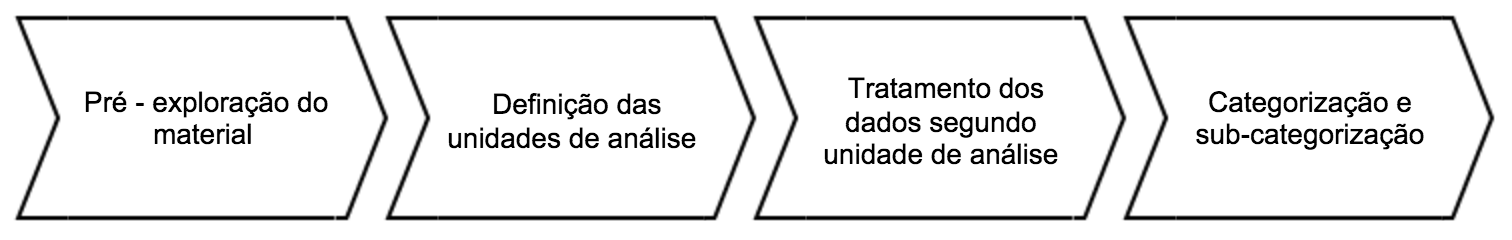
\includegraphics[scale=0.5]{img/fasesanalisedeconteudo}}
\label{fig:fasesanalisedeconteudo}
\caption* {Fonte: Simplificação do modelo \citeonline{bardin} realizada pelo autor}
\end{figure}

A fase inicial de pré-exploração tem como principal objetivo conhecer o contexto do material a ser analisado, retirar impressões e orientações para a próxima etapa. Um dos principais mecanismos dessa etapa é a leitura flutuante, que permite um primeiro contato com o conteúdo do "corpus de análise", raso o suficiente para gerar a formulação de algumas hipóteses e não tomar tempo excessivo do analista. A leitura menos aderente permite a assimilação do "corpus de análise" de forma não-estruturada permitindo a transcendência da mensagem de forma explícita para visualizar pistas não inicialmente óbvias.

Em seguida, é necessário definir a unidade de análise a ser trabalhada, baseada no conteúdo do material avaliado. Essas unidades podem incluir palavras, frases, parágrafos, textos inteiros, de tal forma que possa ser feito algum tipo de análise utilizando-as. A partir das inferências obtidas na etapa anterior, é possível que já tenha sido visualizado que tipo de análise ou categorização poderia ser feito posteriormente, dependendo do tipo de dado analisado. Quando há uma grande repetição de informação devido a um escopo fechado de cada mensagem, é possível utilizar palavras ou frases como unidade de análise para uma posterior análise frequencial. Para os casos em que há uma diversidade maior de informação, a utilização de trechos maiores de texto permitem uma análise temática, a fins de categorização posterior.

Como pode se tratar de um grande volume de dados, é possível que haja a necessidade de um tratamento desses dados de forma a chegar em representações condensadas e explicativas. Para textos maiores, seria oportuno coletar somente as partes relevantes que explicam o conteúdo da própria mensagem passada. Já para palavras e frases, é possível que ocorram palavras sinônimas e frases com o mesmo conteúdo semântico, que tratadas dentro de um mesmo contexto facilitariam a sua categorização posterior. Dentro desse contexto, softwares simples de contagem de palavras até outros mais complexos baseados em algoritmos de \textit{Machine Learning} ganham um espaço de atuação muito grande nessa área, por agilizar esse tipo de tratamento.

Finalmente, através do tratamento desses dados, é possível segmentar as unidades de análise em categorias e em sub-categorias, se necessário. O nível de granularidade ou o gênero dessas categorias deve variar segundo os pontos que querem ser abordados na análise, entretanto recomenda-se fazer a categorização em um nível mais granular, para poder ser feita uma recategorização em níveis menos granulares posteriormente, se necessário.

\subsection{Análise SWOT}
\label{cha:analise_swot}

A análise SWOT é uma ferramenta utilizada para analisar o ambiente e o contexto em que uma empresa se encontra posicionada diante do mercado. O processo de utilização consiste basicamente em organizar características da empresa e do ambiente em que se encontra em quatro principais avaliações: Pontos Fortes (\textit{Strengths}), Pontos Fracos (\textit{Weaknesses}), Oportunidades (\textit{Opportunities}) e Ameaças (\textit{Threats}), conforme quadro ilustrado abaixo. Essa modalidade de análise tem como principal vantagem a simplificação de uma estrutura complexa apresentada por uma organização, facilitando na tomada de decisões estratégicas.

\begin{figure}[H]
\caption{Quadro SWOT básico}
\centerline{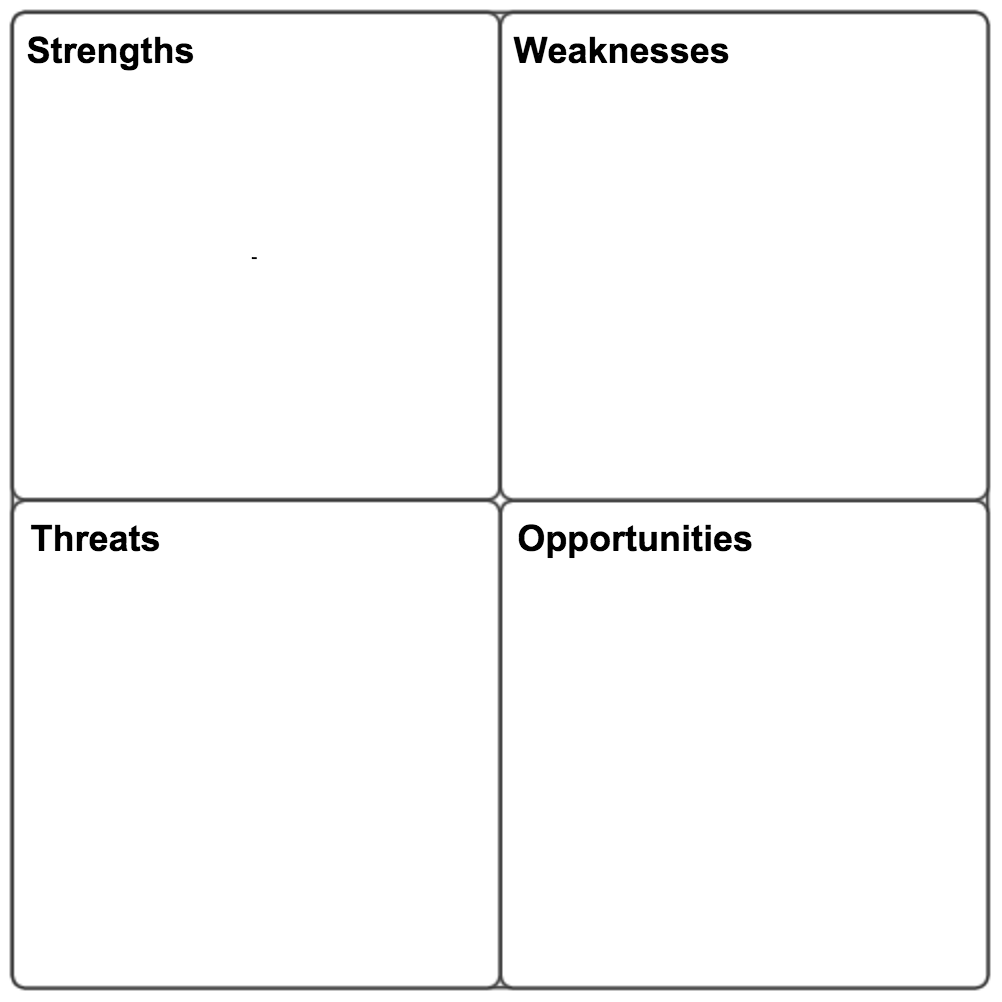
\includegraphics[scale=0.5]{img/detailedswot}}
\label{fig:detailedswot}
\caption* {Fonte: Quadro SWOT básico}
\end{figure}

\section{Método}

\label{chap:metodologia}

\begin{figure}[h]
\caption{Metodologia Utilizada no Trabalho}
\centerline{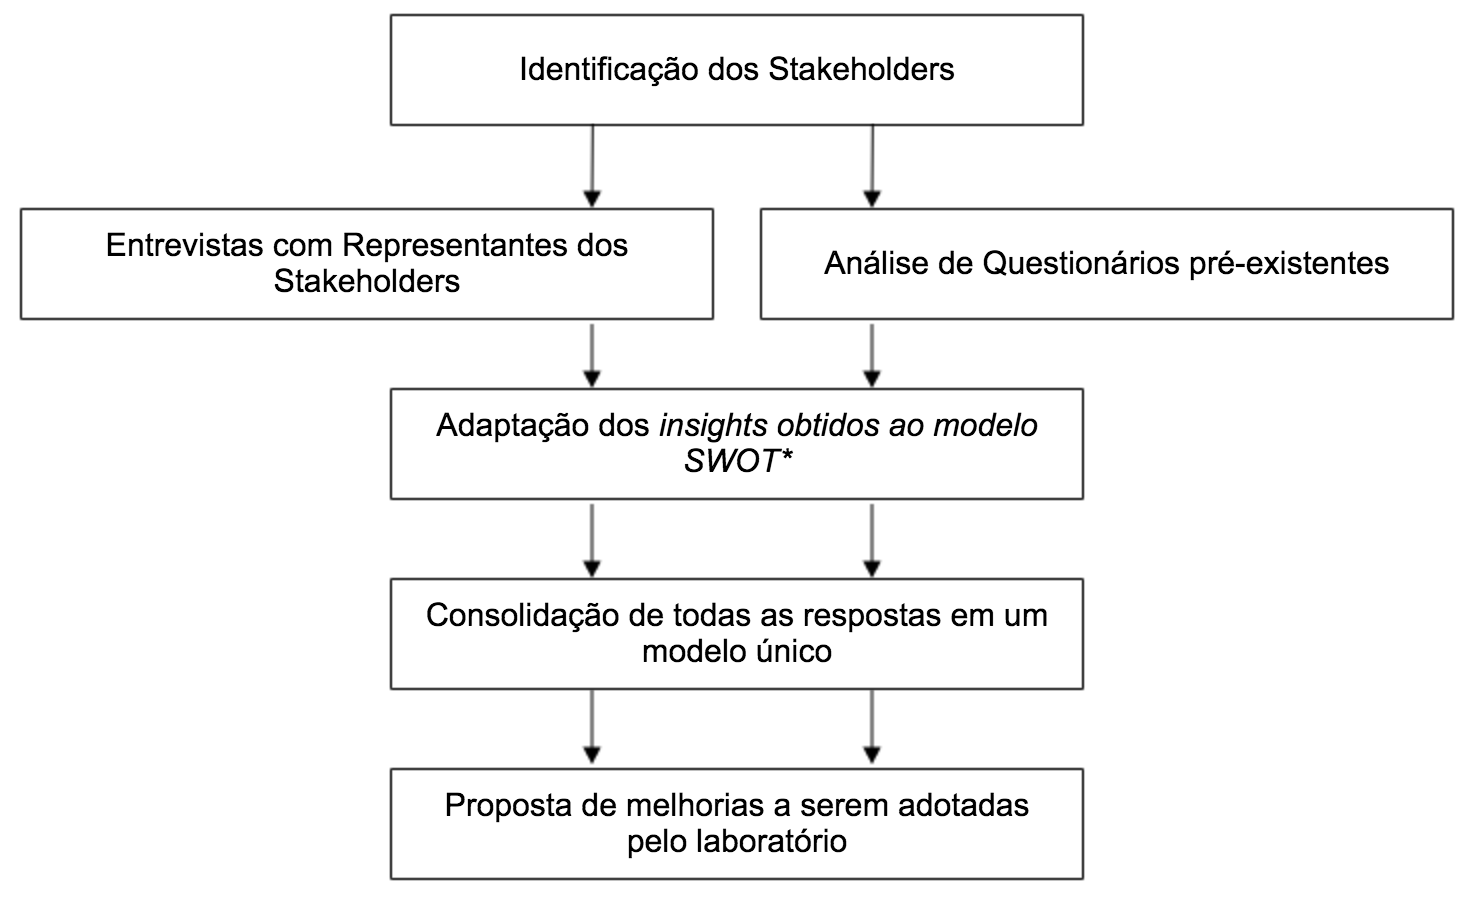
\includegraphics[scale=0.5]{img/metodologia}}
\label{fig:metodologia}
\caption* {Fonte: Elaborado pelo próprio autor}
\end{figure}

Após conversas iniciais com membros da Samsung e do PRO, foram definidos os stakeholders do projeto Ocean, juntamente com as pessoas-chave de cada. Foram realizadas entrevistas semi-estruturadas e gravadas, de forma a permitir a liberdade para serem feitas perguntas não presentes na estrutura inicial, e assim ter uma conversa guiada com o entrevistado como se não fosse uma entrevista formal. Antes de cada entrevista eram preparadas perguntas relacionadas ao mapeamento e percepção das interações do \textit{stakeholder} com o Ocean segundo a visão do entrevistador, e para todos os entrevistados era perguntado "se a pessoa teria alguma sugestão para a melhoria do Laboratório".

Para análise de um \textit{stakeholder} em particular, representado pelo alunos dos cursos básicos do programa Ocean que serão apresentados nesse capítulo, o método de entrevistas foi considerado menos eficiente pelo alto número e rotatividade de alunos. Juntamente a este fato, a Samsung tinha uma necessidade de analisar questionários de \textit{feedback} respondidos nos últimos dois anos de cursos, que nunca haviam sido analisados diante das suas questões qualitativas, apenas das quantitativas. Dessa forma, foram unidas as necessidades de ambas as partes e foram aproveitados esses questionários - totalizando um total de 5280 respostas - para extrair as informações necessárias para este trabalho. O modelo de questionário aplicado encontra-se em anexo. No caso, foram analisadas somente as respostas das questões analíticas: "O que mais o motivou nesse curso?", "O que você acha que pode ser melhorado?" e "Qual tema você gostaria que fosse abordado num próximo curso?".

De forma a analisar e extrair informações desses questionários, o autor optou por desenvolver um software próprio (https://github.com/GabrielArakaki/wordAnalysis) para manipular esses dados via palavras-chave, pelos motivos elencados a seguir.

\begin{description}
\item [Volume de Dados] A quantidade de dados é grande o suficiente para dificultar - porém não inviabilizar - a leitura individual de cada uma das respostas. Acredita-se que mesmo que se optasse pela leitura individual, ela deveria ser acompanhada de uma \textit{clusterização} das respostas em categorias, o que a análise via repetição de palavras-chave também permite encontrar. Em contrapartida, os dados são suficientemente pequenos a ponto de não ser viável buscar alternativas  de \textit{Machine Learning} existentes para tratar esses dados, pois o volume não seria suficiente para treinar a inteligência artificial utilizada.

\item [Proposta do Estudo] Embora exista um campo muito grande de possibilidades de tratar e manipular os dados presentes, existe a necessidade de seguir com os objetivos inicias do presente estudo, que diz respeito ao estudo do projeto Ocean de forma holística, e não somente na questão do aprendizado transmitido através de seus cursos. O autor acredita que há espaço para análises mais sofisticadas - dignas de um trabalho dedicado somente a isso - que poderiam ser realizadas caso a Samsung encontre a necessidade de entender os cursistas nos mínimos detalhes.

\item [Manipulação de Dados] O uso de uma ferramenta própria dá ao autor a liberdade de trabalhar e iterar em cima dos dados de forma a otimizar a ferramenta para o próprio uso. Existem disponíveis ferramentas prontas de geração de nuvens de palavras, que possuem um intuito muito maior de apresentar um 'choque visual' do que apresentar dados analíticos em si. A manipulação de dados permite que o autor encontre associações entre palavras ao observar os dados gerados pela ferramenta e trabalhar em cima da própria ferramenta para eliminar redundâncias ou dados inconsistentes.

\item [Desenvolvimento Ágil] O desenvolvimento ágil é um \textit{framework} de desenvolvimento de software que possui o intuito de permitir o desenvolvimento em um curto período de tempo com um iterações feitas através da coleta de \textit{feedbacks} de forma rápida e sistemática. No caso deste trabalho, o autor não encontrou uma ferramenta que fornecesse customização e flexibilidade conforme suas necessidades, fazendo com que optasse por desenvolver um software próprio. Não obstante, é de satisfação do autor como desenvolvedor utilizar programação para resolver problemas reais.
 
\end{description}

Para consolidar a análise realizada para cada \textit{stakeholder}, foi utilizada uma adaptação do modelo SWOT para ilustrar as percepções obtidas de cada um. Ela difere do modelo original do SWOT por não se tratar de uma análise de negócio baseada em fatores de mercado e competitividade com outros \textit{players}, e sim em uma análise fria e absoluta de fatores básicos em um projeto: Pontos Fortes, Pontos Fracos, Oportunidades e Ameaças. Foi considerado que por ser um modelo simples e de fácil visualização, consolidaria as necessidades deste trabalho sem desvirtuar os objetivos propostos.

A partir dos resultados obtidos pela análise das respostas, trabalhou-se em cima da geração de propostas de melhoria.

\section{Identificação de Stakeholders do Laboratório}
\label{sec:identificacao_stakeholders}

A partir de conversas informais com os professores mais próximos ao projeto Ocean e com os próprios responsáveis da Samsung pelo laboratório, foi possível desenhar um mapa ilustrativo para os principais \textit{stakeholders}.

\begin{figure}[H]
\caption{Mapa de stakeholders do projeto Ocean}
\centerline{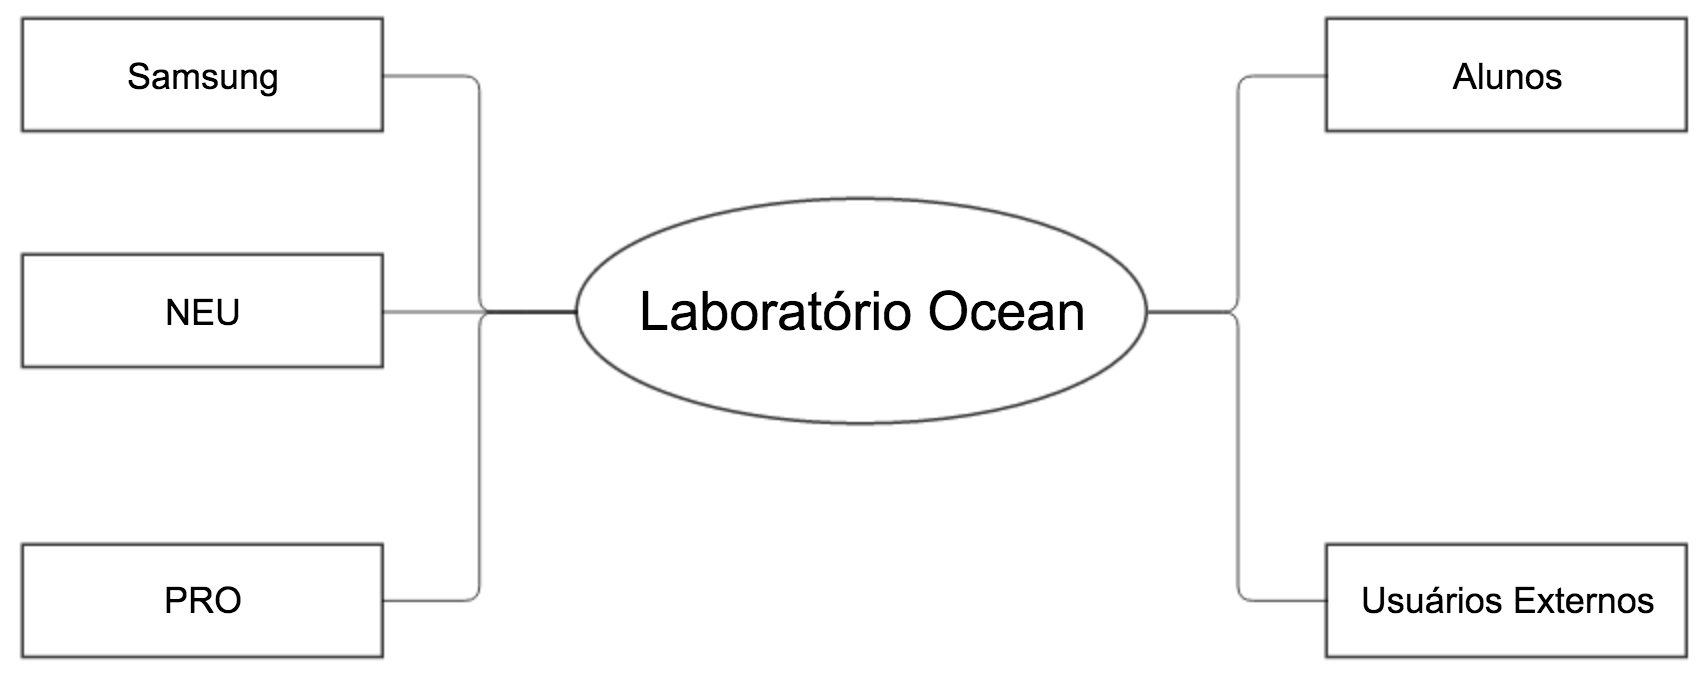
\includegraphics[scale=0.5]{img/stakeholders_v2}}
\label{fig:stakeholders}
\caption* {Fonte: Elaborado pelo próprio autor}
\end{figure}

Em um segundo momento foram definidos as principais fontes de dados para cada um dos \textit{stakeholders}, assim como os principais métodos de coleta, sendo definido o aproveitamento de questionários já respondidos pelos cursistas básicos e entrevistas para os demais.

\begin{figure}[H]
\caption{Pontos de contato dos \textit{stakeholders}}
\centerline{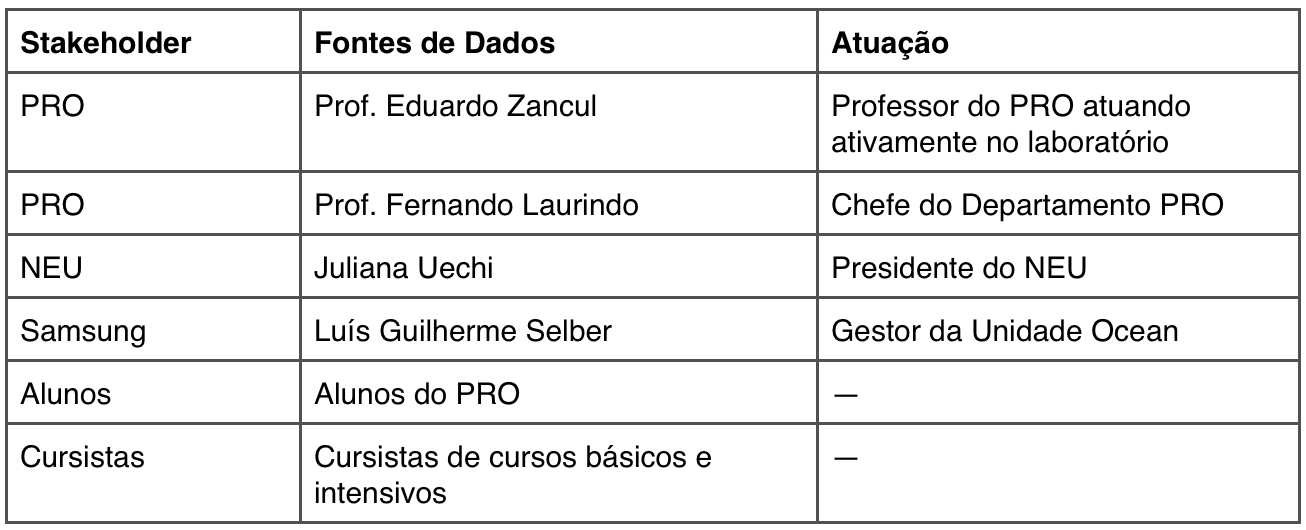
\includegraphics[scale=0.6]{img/stakeholderspoc}}
\label{fig:stakeholderspoc}
\caption* {Fonte: Elaborado pelo próprio autor}
\end{figure}


\subsection{PRO}
\label{sec:con_pro}

O Ocean é um dos quatro grandes projetos que o PRO acompanha atualmente, esquematizado pela Tabela \ref{tab:pilares_pro}, juntamente com Inovalab, a Fábrica Didática e o Núcleo de Empreendedorismo da USP.

\begin{table}[H]
\begin{center}
\caption{Pilares do PRO}
\label{tab:pilares_pro}
{\def\arraystretch{2}\tabcolsep=10pt
\begin{tabular}{>{\raggedright}p{0.2\linewidth}>{\raggedright\arraybackslash}p{0.2\linewidth}>{\raggedright\arraybackslash}p{0.2\linewidth}>{\raggedright\arraybackslash}p{0.2\linewidth}}
\hline
     & Objetivo Institucional & Participação do PRO & Em Atividade  \\ \hline
     Inovalab & Laboratório de Inovação & Gestão Ativa & Sim  \\
     Fábrica Didática & Apropriação de conceitos de fábricas para aplicação no ensino & Em Desenvolvimento & Não \\
     Ocean & Laboratório de Desenvolvimento de Software & Cogestão com a Samsung & Sim \\
	 Núcleo de Empreendedorismo da USP & Disseminação da cultura empreendedora & Cede espaço físico & Sim \\ \hline
\end{tabular}%
}
\caption* {Fonte: Elaborado pelo autor em conversa com professores do departamento}
\end{center}
\end{table}

O Inovalab é um laboratório que oferece recursos para realização de projetos de engenharia, como \textit{software}, \textit{hardware}, impressoras 3D e oficinas mecânicas. A infraestrutura do laboratório é utilizada para sediar o NEU, outro dos projetos que será discutido adiante. Já a Fábrica Didática é um projeto que consiste na produção de peças e produtos com a perspectiva de gerar pesquisa na área de fabricação e ensino para os alunos da engenharia de produção.

O que pode se ver em comum entre esses projetos e o Ocean é a proximidade da inovação e do empreendedorismo, pontos que o PRO considera essenciais para a tríade pesquisa, ensino e extensão. A Engenharia de Produção na Poli propicia um ambiente de aprendizado com disciplinas que já contribuem nessa área, como Projeto Integrado e Desenvolvimento de Produto, porém grande parte do aprendizado pode ser obtido através de atividades extra curriculares, propiciadas em parte por esses projetos. Um dos principais métodos de aprendizagem que a Poli incentiva nos alunos é o \textit{self-learning}, pois a área de Engenharia cobre uma variedade tão extensa de temas que o aluno que tiver interesse em se aprofundar em temas específicos deve buscar conhecimento por conta própria, sendo o principal papel da faculdade fornecer uma base sólida e uma estrutura para que ele possa adquirir conhecimento com facilidade.

\subsection{NEU}
\label{sec:con_neu}

O Núcleo de Empreendedorismo da USP é uma organização formada por alunos de graduação e pós-graduação, pesquisadores e professores que possuem a missão de promover a cultura de empreendedorismo dentro da Universidade. O NEU é aberto à toda comunidade da USP, já tendo recebido contribuições de diversas instituições da universidade, porém é formado atualmente principalmente por alunos da POLI e da FAU.

De forma similar ao estabelecimento do Ocean dentro do departamento do PRO, o NEU foi convidado a utilizar o espaço do Laboratório de Inovação (InovaLab) para sediar suas atividades. Atualmente o NEU trabalha com três principais pilares: inspiração, capacitação e conexão.

Inspiração diz respeito ao fomento ao empreendedorismo nos alunos para que eles se sintam impulsionados a participar do ecossistema de \textit{startups} ou até abrir as suas próprias. Portanto são feitos diversos convites aos diretores de diversas \textit{startups}, muitos com origens da própria USP, como Lean Survey, 99 Táxis e Squid, e estes podem explicar um pouco da sua trajetória e das emoções vividas graças aos seus empreendimentos. 

Capacitação é a frente do NEU de auxiliar ideias de alunos a se desenvolverem em produtos, para que assim sejam criadas novas empresas. A partir da rede de empresas que o NEU tem em seu leque de contatos, ele consegue encontrar mentorias para as empresas e acelerar o seu desenvolvimento. O principal programa dessa frente é o \textit{Startup Lab}, em que o NEU fornece material de apoio e mentoria através dos seus contatos com empresas, investidores e aceleradoras.

Conexão é representado principalmente pelo \textit{Startup Ship}, que é o canal do NEU destinado a alunos que querem estagiar em \textit{startups}. Através de sua rede de conexões ela facilita com que \textit{startups} e os alunos certos cheguem uns aos outros. Outro programa é o Pesquisas USP, que auxilia os alunos a se conectarem com pesquisas, e em contrapartida auxiliar pesquisadores a se conectarem com alunos ou empresas que possam auxiliar nos seus estudos. Nesse programa o NEU também auxilia startups a entrarem em contato com aceleradoras.

O NEU apresenta uma sinergia muito grande com o Ocean, pois ambos possuem muito interesse nessa fase de pré-aceleração de empresas, conseguindo exercer etapas distintas e complementares nesse processo. Durante os cursos intensivos do Ocean, o NEU se responsabiliza por trazer contatos de diferentes empresas para inspirar e fazer mentorias, ao passo que a Samsung trabalha fortemente na parte de capacitação e acompanhamento da evolução das empresas ao longo do programa.

Existe uma série de organismos dentro da universidade que fomentam a cultura de empreendedorismo, e como todos são gratuitos, existe uma colaboração muito grande para que os maiores beneficiados sejam as \textit{startups}, independente de  qual instituição que esteja contribuindo mais para a evolução da empresa.

\subsection{Alunos}
\label{sec:con_alunos}

A Engenharia de Produção é uma área que tem suas origens na engenharia mecânica, pois a formação de engenheiros no passado era voltada principalmente à capacitação técnica de produção de peças e produtos, sem um estudo aprofundado de como fabricá-los com eficiência. Os estudantes eram ensinados a desenhar um produto e desconstruí-lo em diversas peças que deveriam atuar conjuntamente para o funcionamento desejado. Encontrou-se então uma oportunidade de criar um novo ramo da Área Mecânica que se encarregaria de capacitar os alunos a aplicar conceitos de fábrica utilizados globalmente, como otimização das linhas de produção, controle da qualidade e controle da produção, não explorados anteriormente nos cursos de engenharia. Inicialmente voltado principalmente ao setor automotivo, a área de produção começou a ser expandida para poder aplicar os mesmos conceitos de fábrica para qualquer indústria, exigindo uma abstração dos principais conceitos, e inclusive a adoção de teorias de administração e gestão de projetos.

Atualmente, duas disciplinas eletivas estão utilizando a infraestrutura do laboratório, Desenvolvimento Integrado de Produto e Criação de Negócios Tecnológicos, porém o laboratório cede seu espaço a disciplinas que necessitem dos seus recursos. Muitas das reclamações dos alunos em relação ao ensino atual diz respeito às aulas que são passadas utilizando tecnologias antigas, como retroprojetores. Embora o laboratório não esteja sendo usado pelas disciplinas obrigatórios, os alunos enxergam que a sua presença eleva o patamar de tecnologia de ensino a ser utilizado, o que no curto ou médio prazo pode abandonar as tecnologias antigas para adotar o maior uso de mídias digitais.

Além da questão das disciplinas, o laboratório é utilizado pelos alunos durante o período fora da aula, para a realização de trabalhos , tarefas ou para fixar o conteúdo que foi dado em aula. Como o laboratório fica aberto até as 22 horas, e na cultura da engenharia é bastante comum ficar até tarde estudando, alunos utilizam o laboratório praticamente o dia inteiro. Antes do laboratório era frequente os alunos irem estudar em outros departamentos como a Engenharia Civil, que possui várias mesas no seu saguão principal, e ficava aberta até tarde para os alunos de pós-graduação. Embora grande parte dos alunos traz o seu próprio \textit{notebook} para estudar, alguns utilizam os notebooks da própria samsung e até um outro monitor para otimizar as suas tarefas.

A presença de um laboratório como este também ajuda a fomentar a cultura de empreendedorismo dentro da universidade, pois permite a capacitação dos alunos diante do desenvolvimento de produtos, base de criação de novas \textit{startups}. Segundo as pesquisas realizadas por \citeonline{entrepreneurship} com estudantes de graduação de engenharia, a experiência de empreendedorismo é observado de 4 maneiras, independentemente se eles desejam empreender ou não: 

\begin{enumerate}
\item Primeiro passo para o auto-aprendizado
\item Preparação para a vida no trabalho
\item Caminho para ser autônomo
\item Desenvolvimento de liderança e responsabilidade de um time
\end{enumerate}

Como esses pontos seguem na mesma direção dos objetivos da Poli e não agrada somente aqueles alunos que desejam ser empreendedores, o PRO pode continuar fomentando o empreendedorismo para que atinja todos os alunos. Entretanto, de forma a potencializar ainda mais os futuros empreendedores, é necessário entender o perfil daqueles alunos que desejam abrir o seu próprio negócio, como foi observado em diversas pesquisas como a realizada por \citeonline{empreendedorismo}, em que identifica o perfil de alunos que são atraídos pelo empreendedorismo:

\begin{itemize}
\item Propensão a assumir riscos
\item Proximidade a outros empreendedores no círculo próximo
\item Já possuem uma ideia desenvolvida para o empreendimento
\end{itemize}


\subsection{Cursistas}
\label{sec:con_cursistas}

Conforme explicado anteriormente, o Ocean trabalha com duas propostas de cursos, os cursos básicos e os cursos intensivos. O primeiro grupo corresponde à capacitação de desenvolvedores para que gerem conteúdo através de \textit{software} para dispositivos da Samsung, já o segundo é para pessoas que desejam empreender e possuem uma ideia inicial para ser desenvolvida. Embora exista uma gama de pessoas que seja usuária de ambos os cursos - os novos empreendedores têm muito interesse por programação - o público-alvo de cada um é diferente.

Os cursos básicos são desenhados para programadores ou aspirantes à programação. Embora existam diversos temas de cursos, o principal objetivo da Samsung consiste em capacitar os cursistas a explorarem todas as funcionalidades permitidas pelos \textit{hardwares} da Samsung. Para isso, são explorados o sistema operacional Android, os SDKs da Samsung, o sistema operacional Tizen, em suma tudo que possa contribuir para que o desenvolvedor possa gerar valor e conteúdo sem se preocupar em desenvolver um hardware específico. Portanto, é um curso de bastante interesse para iniciantes que desejam iniciar o aprendizado em programação, para desenvolvedores experientes que não tiveram muito contato com dispositivos móveis até para apaixonados pela Samsung que querem verificar na prática todo potencial permitido pelos seus dispositivos.

Segundo a 27\textsuperscript{a} Pesquisa de Anual do uso de TI, realizada pela Fundação Getúlio Vargas (FGV), o número de smartphones em uso no Brasil gira atualmente em torno de 168 milhões de dispositivos. \cite{tifgv}. Não obstante, além do alto número de smartphones, o Brasil também se mostra presente no mercado de outros dispositivos inteligentes, com previsão de movimentação de US\$4,1 bilhões no Brasil com IOT, segundo a assessoria de imprensa da IDC Brasil. \cite{idc}. Segundo a ONG Code.org, financiada por fundadores das maiores empresas de tecnologia do mundo como Mark Zuckerberg e Bill Gates, o número de empregos para programadores cresce exponencialmente, ao passo que o ensino de programação nas escolas não acompanha o mesmo ritmo, o que gerará uma falta de profissionais de TI em um futuro próximo. Juntamente a essa informação, o departamento de estatísticas de trabalho dos Estados Unidos (\textit{Bureau of Labor Statistics}) estima que o número de empregos para programadores fora dos EUA para trabalho remoto aumentará consideravelmente. \cite{bls}

É nesse cenário de alto crescimento do uso de novas tecnologias no Brasil que o mesmo se mostra como um grande mercado para produtos inerentes ao uso de dispositivos inteligentes, como aplicativos e games. Dentro desse contexto, jovens interessados pelo desenvolvimento desse mercado no país se interessam por propostas como a do Ocean para realizar diferentes cursos nessas áreas.
 
O segundo tipo de curso - cursos intensivos - foram feitos para incentivar ideias a se tornarem empresas, então é voltado para o nicho empreendedor. De acordo com o projeto \textit{Global Entrepreneurship Monitor}, que realiza pesquisas anuais sobre empreendedorismo no mundo, estima-se que em 2015, 52 milhões de brasileiros com idade entre 18 e 64 anos se envolveram na criação ou manutenção de algum negócio. Entre 2015 e 2014, houve um salto do total de empreendedores entre pessoas de 34,4\% para 39,9\% da população da faixa etária mencionada, principalmente devido ao surgimento de novas empresas. \cite{GEM}

Uma pequena parte dessas empresas é constituída de empresas com alto valor agregado e/ou com produtos de alta tecnologia, porém é visível o aumento da procura de pessoas que possuem ideias e buscam algum tipo de mentoria para desenvolvê-las a ponto de poder empreender. É nesse momento em que elas encontram o Ocean, onde podem utilizar de toda \textit{expertise} da Samsung para desenvolver um produto ou serviço de alta qualidade. Portanto não é necessário que os grupos já possuam uma empresa e um produto em funcionamento, até porque o programa desses cursos envolve questionar e validar hipóteses a respeito do próprio modelo de negócio da empresa, independente da maturidade da ideia. 

Os cursos intensivos são de uma extensão muito maior, e exigem uma intensidade muito grande dos cursistas, com reuniões de três horas de segunda à quinta-feira. Esse fator mostra a seriedade do programa em trabalhar com pessoas que mostrem um comprometimento acima da média, até porque muitos dos cursistas possuem emprego fixo e devem arranjar um tempo para se dedicar ao programa. Não obstante, além de ter esse acompanhamento quase diário nos dias úteis, são definidas metas semanais a serem cumpridas, para guiar as equipes no seu planejamento da semana. Toda essa intensidade tem o objetivo de deixar os alunos engajados ao longo do curso, que por ser gratuito e não exigir participação societária por parte da Samsung, pode facilmente ser abandonado se o aluno não observar o comprometimento da própria empresa.
%!TEX root = index.tex
\chapter{Analises}
\label{cha:analises}

A seguir são apresentadas as análises realizadas com cada um dos \textit{stakeholders}, ilustradas por uma análise SWOT. Cada um deles apresenta uma série de particularidades, tanto na coleta quanto na análise dos dados obtidos, porém todos fornecerem dados valiosos para esse trabalho.

\section{Samsung}

Em entrevista realizada com o gestor da unidade Ocean, Luís Guilherme Selber, o laboratório vive um momento sem muitos problemas, principalmente pelo fato de o projeto estar em uma fase inicial. Não há formalidades estabelecidas como reuniões periódicas, pois quando é necessário realizar um alinhamento com o departamento é fácil encontrar um professor no corredor ou em sua sala, portanto as interações se limitam às necessidades de um ou outro, sem conflitos até o momento. A própria gestão de uso do laboratório compartilhada entre as atividades do Ocean/Samsung e o PRO não gera conflitos pois as necessidades de uso do laboratório por cada parte já foram previamente estabelecidas e esclarecidas nas reuniões iniciais de fechamento do projeto.

Segundo Selber, o laboratório sofreu uma mudança muito positiva devido à mudança de localidade para dentro da universidade. A presença do laboratório dentro do PRO mudou completamente a utilização do laboratório, que agora é ocupado das 08 da manhã até as 22 da noite de segunda a sexta, fato que não acontecia na antiga sede. Quando era localizado na Av. Brigadeiro Faria Lima, a Samsung exercia um papel ativo de sediar eventos próprios ou externos com o intuito de divulgar e preencher o espaço do laboratório, pois quanto mais pessoas utilizassem o espaço maior seria a divulgação indireta do programa e dos cursos oferecidos pelo laboratório. Não obstante, além dos próprios cursos dados pelo laboratório, ainda existe um investimento por parte da empresa com equipamentos, internet e infraestrutura que não deveria ser desperdiçado. Outra grande vantagem de estar dentro da universidade consiste no fato de a USP ser um ecossistema de parcerias com diversas empresas. Dentro desse meio, a Samsung viu uma oportunidade de expandir sua rede de contatos com outras empresas, o que já trouxe bons resultados até o momento, com reuniões realizadas com outras grandes empresas do mercado nacional. A universidade também propiciou o aumento de demanda pelos cursos básicos e intensivos, com um grande aumento principalmente entre alunos da universidade. A proximidade com o NEU e a POLI permite uma divulgação muito mais fácil do laboratório na universidade.

A Samsung enxerga algumas oportunidades a serem exploradas pelo laboratório, como uma maior participação de professores nos cursos do laboratório, seja através de aulas ou mentorias. Eles acreditam que existe uma sinergia muito boa entre academia e empresa no sentido de engajar e incentivar os alunos dos cursos a buscarem mais conhecimento nas suas áreas de interesse. Outra oportunidade citada por Selber seria buscar uma adesão maior aos cursos e ao próprio dia a dia do laboratório por parte de outras instituições da Universidade. Tanto a Faculdade de Economia, Administração e Contabilidade (FEA) quanto o Instituto de Matemática e Estatística (IME) por suas formações ligadas ao empreendedorismo e ao desenvolvimento de software mostram ser muito compatíveis com os programas oferecidos pelo Ocean, entretanto a grande maioria de adeptos vêm da Escola Politécnica.

A partir dos pontos levantados anteriormente, foi construída a seguinte análise:

\begin{figure}[H]
\caption{Análise do Ocean - Samsung}
\centerline{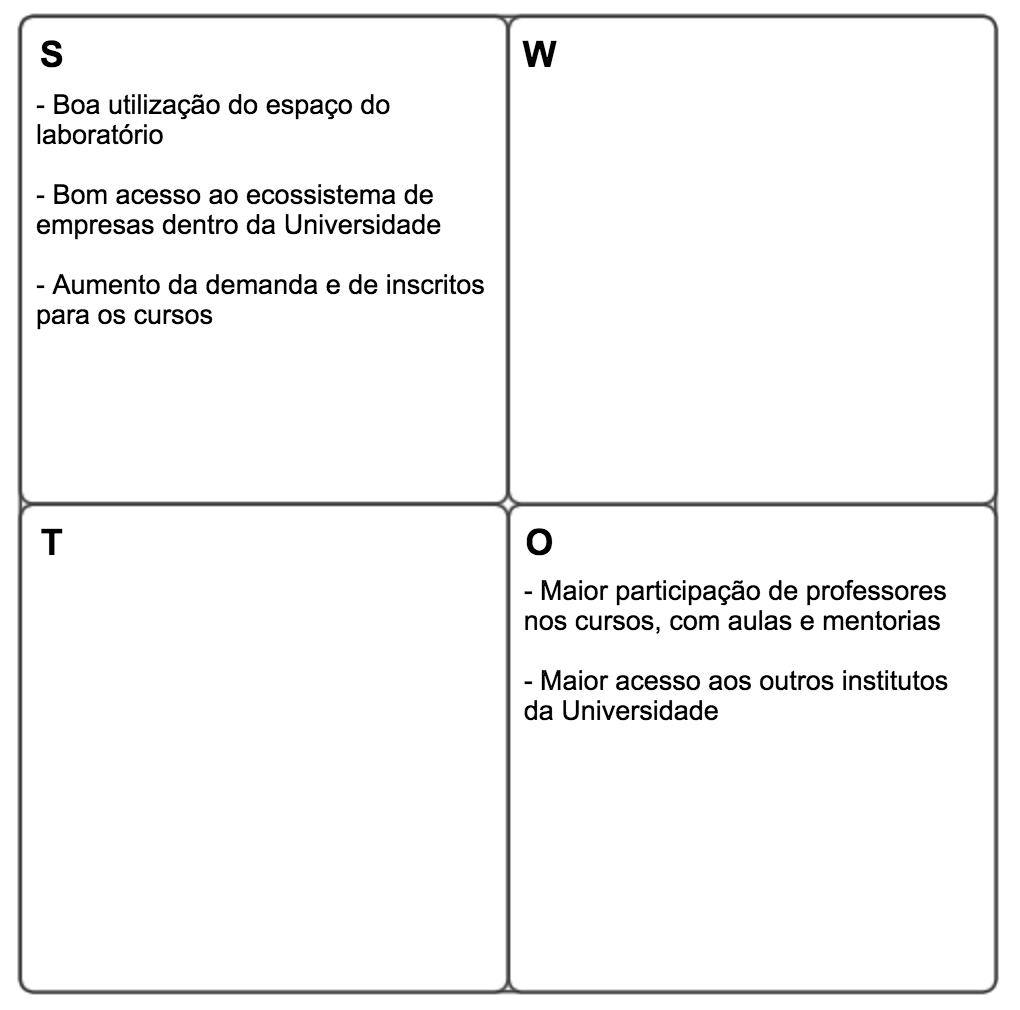
\includegraphics[scale=0.75]{img/samsungswot}}
\label{fig:swotsamsung}
\caption* {Fonte: Elaborado pelo próprio autor}
\end{figure}

\section{PRO}

Para a obtenção dos dados relacionados ao PRO, foram entrevistados o professor Fernando Laurindo - chefe do departamento - e o professor Eduardo Zancul, que possui participação ativa no laboratório Ocean e no InovaLab. 

Em um primeiro momento, a parceria com o Ocean é vista como um projeto de investimento externo aplicado ao departamento e à universidade que surgiu e foi executado com muita rapidez. Entre as conversas iniciais e o final da reforma da área do laboratório foram cerca de 4 meses. Esses fatores são consequência do comprometimento por parte tanto do departamento, que agilizou toda burocracia para permitir a criação do laboratório, quanto por parte da Samsung, que se encarregou e custeou toda construção do laboratório. Esse comprometimento se deu principalmente pela sinergia do projeto Ocean dado ao ecossistema de inovação e empreendedorismo que cresce cada vez mais dentro da universidade e a vontade da Samsung de se aproximar cada vez mais da comunidade estudantil.

Para o professor Eduardo Zancul, existe uma clara conexão estratégica entre o Ocean, o InovaLab e os outros projetos do departamento e para ele, esse foi um dos principais fatores que despertaram na Samsung o interesse de mover o laboratório para dentro da universidade. Foi através do Inovalab que foi feito o primeiro contato com a Samsung, e o NEU colabora ativamente com os cursos intensivos do Ocean, trazendo mentores e palestrantes para auxiliar nos cursos. Dentro desse ecossistema de projetos geridos pelo PRO, o laboratório Ocean representa o elemento tecnológico - em especial dispositivos móveis, realidade virtual, \textit{games} e internet das coisas - e a capacitação técnica para desenvolver projetos nessas frentes, incentivando os projetos que surgem no InovaLab e no NEU. Dessa forma, projetos de inovação podem gerar projetos de empreendedorismo ou pessoas interessadas por inovação podem se engajar por projetos de empreendedorismo com maior facilidade.

O empreendedorismo, em particular, sempre acompanhou a trajetória de alunos da Poli que optaram por abrir a sua própria empresa ao invés de entrarem no mercado de trabalho através do recrutamento de empresas. Não obstante, muitas empresas tiveram o desenvolvimento de seu modelo de negócio realizado em paralelo ao trabalho de graduação de alunos. Por isso a Poli busca sempre oferecer recursos que forneçam a estrutura necessária para os alunos buscarem o seu aprendizado.

À parte da relação com outros projetos, uma das principais discussões sobre o laboratório gira em torno de como utilizá-lo para incentivar as frentes de pesquisa, ensino e extensão baseado nas propostas do laboratório. Atualmente, o laboratório é utilizado por duas disciplinas optativas do departamento, e está liberado para o uso de qualquer disciplina obrigatória, com a única condição de que o formato da aula apresente uma demanda da infraestrutura do laboratório, senão o PRO disponibiliza uma sala de informática com os equipamentos necessários, porém com menor sofisticação do que o Ocean.

Entretanto como ainda está em fase inicial, não houve tempo para os pós-graduandos começarem a utilizar o espaço e iniciar as pesquisas, sendo essa a maior oportunidade de desenvolvimento do laboratório, que segundo os professores acontecerá inevitavelmente, é apenas uma questão de algum aluno se disponibilizar a fazer algo relacionado ao Ocean.

Como parceiro de cogestão do Ocean, o PRO é dono e responsável pelo espaço do laboratório e pode utilizá-lo conforme sua necessidade, incluindo aulas, palestras, seminários, eventos internos e até eventos externos, se houver a oportunidade. Por via de regra, o PRO pode ceder o espaço a eventos ligados a outras universidades ou a entidades sem fins lucrativo. Caso não se enquadre nesses dois casos mencionados o PRO pode alugar o espaço a um baixo custo, de forma a arrecadar recursos para o departamento.

A partir das conversas com os professores, foi criada a seguinte análise:

\begin{figure}[H]
\caption{Análise do Ocean - PRO}
\centerline{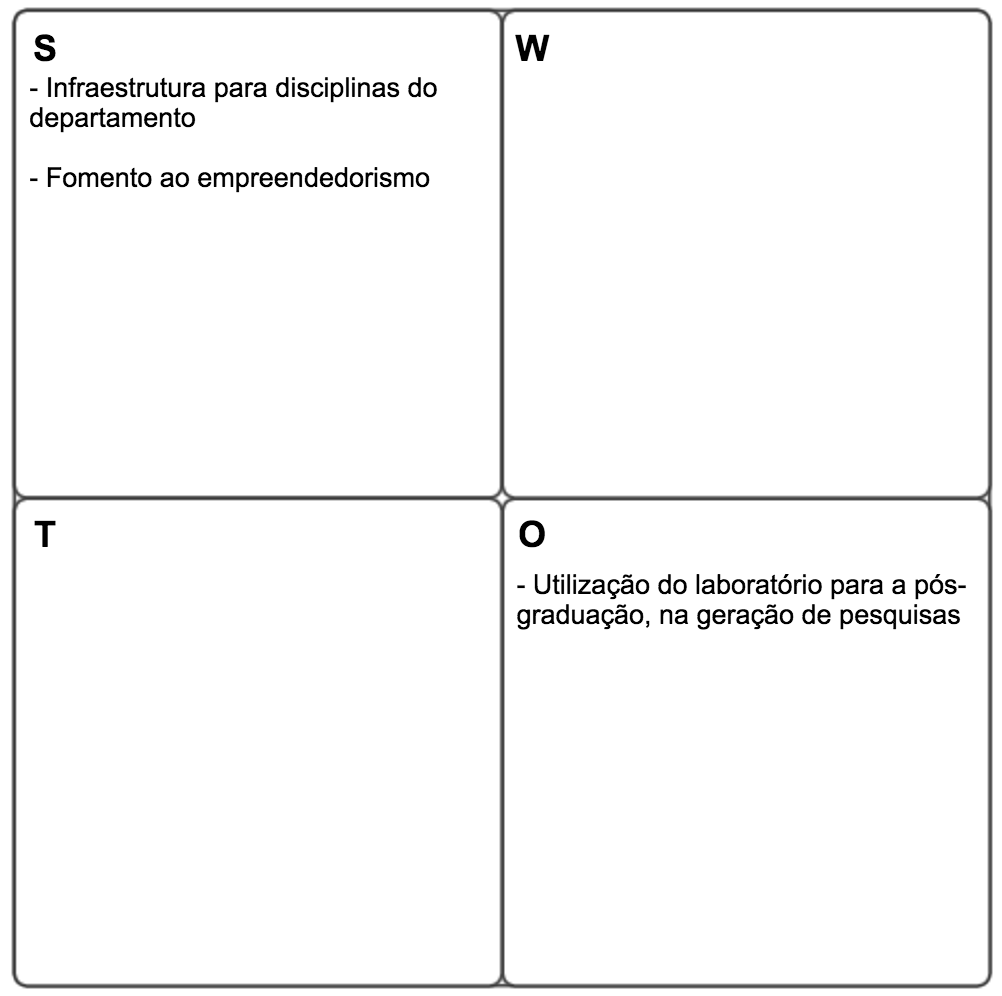
\includegraphics[scale=0.75]{img/proswot}}
\label{fig:swotpro}
\caption* {Fonte: Elaborado pelo próprio autor}
\end{figure}

\section{NEU}

Segundo Juliana Uechi, atual responsável pelo funcionamento do NEU, a presença do Ocean por si só já contribui com o fomento à cultura de empreendedorismo dentro da Universidade, principal objetivo do NEU. Isso porque ainda existe uma carência de motivação pelo empreendedorismo, ainda mais em tempos de crise, a qual encontra no Ocean uma ferramenta gratuita com suporte à pré-aceleração de empresas. 

Atualmente existe uma colaboração ativa entre NEU, PRO e Samsung, principalmente em relação ao atual módulo de curso intensivo do laboratório, que envolve participação de todas as partes. De forma geral, a Samsung é responsável pelo acompanhamento do programa e pela capacitação, e o NEU e o PRO utilizam de suas conexões para trazer mentores às empresas participantes, normalmente ex-alunos que abriram as próprias empresas. Tais colaborações poderiam, segundo Juliana, ir além da participação nos cursos intensivos, porém a agenda de ambas as instituições encontra-se lotada

Em relação à infraestrutura do laboratório, o NEU acredita que o uso do laboratório é subutilizado quando cursos não estão acontecendo. O cenário atual de funcionamento é similar ao de uma biblioteca ou uma sala pró-aluno, onde alunos vão com tarefas individuais ou materiais de estudo, o que é de certa forma redundante pois já há uma biblioteca no departamento. Como uma frente de desenvolvimento e empreendedorismo, poderia haver mais espaço para \textit{coworking} e atividades colaborativas dentro do laboratório. Que fosse uma sala que gerasse valor através da discussão, não da absorção individual, que é igualmente importante, mas a biblioteca seria uma lugar mais adequado para esse tipo de atividade.

Por fim, é ressaltado a sinergia entre empresas que colaboram com o fomento à cultura de empreendedorismo, considerando que por mais que compartilhem o relacionamento com \textit{startups} via pré-aceleração, os alunos precisam ser motivados através de métodos diferentes. E pensando sempre no aluno e nas suas futuras empresas, um ambiente com diversas instituições de fomento ao empreendedorismo e aceleração, evita a entrada na universidade de instituições não-gratuitas, seja através de inscrição nos cursos ou via equity das empresas.

A partir da conversa com a Juliana, foi obtida a seguinte análise:

\begin{figure}[H]
\caption{Análise do Ocean - NEU}
\centerline{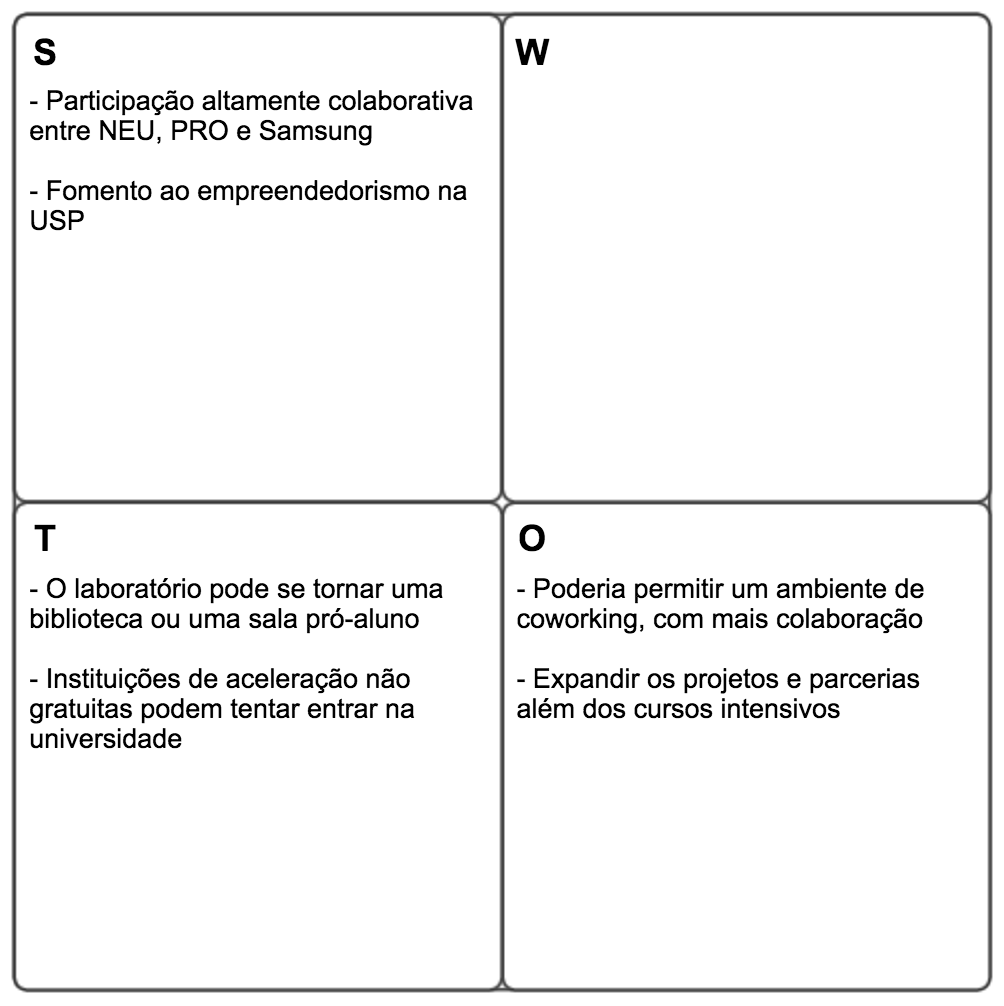
\includegraphics[scale=0.75]{img/neuswot}}
\label{fig:swotneu}
\caption* {Fonte: Elaborado pelo próprio autor}
\end{figure}

\section{Alunos}

De forma a obter as percepções dos alunos diante do laboratório, foram realizadas entrevistas com dez pessoas, entre alunos que frequentavam o laboratório no momento da entrevista e membros do centro acadêmico. Primeiramente, o que se observou em todas as respostas foi uma comparação direta entre o laboratório e duas estruturas do PRO: a biblioteca e a sala de informática. 

A biblioteca atual do departamento funciona de segunda à sexta-feira, das 8h00 até as 18h00, e possui 8 salas para grupos de 4 pessoas, e entre mesas compartilhadas e individuais, possui capacidade para cerca de mais 20 alunos. Parte da biblioteca está interditada por problemas de infraestrutura, que não têm previsão de serem resolvidos, e por ora deixam de abrigar cerca de 30 alunos que poderiam ocupar esse espaço. Para os alunos de engenharia de produção, o laboratório Ocean foi extremamente bem vindo, pois cobre diversos problemas da biblioteca, como o acesso a um wifi de maior qualidade, funcionamento após as 18h e salas da biblioteca cheias. Não obstante, o laboratório ainda possibilita utilizar os monitores com os próprios notebooks, que segundo os alunos são mais utilizados que os notebooks da Samsung.

A sala de informática se localiza em uma antiga sala de aula do departamento, e é utilizada em aulas que demandam o uso de algum \textit{software} ou é necessário a prática de programação, como 'Controle e Automação', 'Modelagem e Simulação de Sistemas de Produção', 'Sistemas de Informação'. Entretanto, segundo alguns alunos, os equipamentos muitas vezes deixam a desejar e atrapalham no acompanhamento das disciplinas. Dado a qualidade dos equipamentos, os alunos prefeririam utilizar os computadores do laboratório para obter maior fluidez nas aulas. Não só, os alunos acreditam que mais aulas poderiam ser informatizadas, como 'Pesquisa Operacional', 'Logística' e 'Finanças', ressaltando que apesar de a prática dessas disciplinas envolverem um uso intensivo de softwares, como Excel e Lingo/Lindo, parte das aulas ainda utiliza retroprojetores para explicações e exercícios. Portanto, os alunos acreditam que o laboratório pode contribuir com a melhoria da dinâmica das aulas.

De forma geral, todos avaliam o laboratório positivamente, porém ressaltaram alguns problemas com a sua utilização. Um dos problemas diz respeito ao processo de utilização do laboratório, pois não há políticas muito claras sobre o uso ou indicações sobre o que é ou não é permitido na sala, principalmente sobre a utilização dos notebooks ou monitores. Também não está claro a quem perguntar para tirar dúvidas, pois não há um monitor na sala. Outro ponto levantado é a falta de algum lugar para consultar se a sala estará disponível para uso com antecedência, relevante para alunos poderem se programar se utilizarão o laboratório ou terão que ir para outro lugar. Por fim, alguns alunos dizem não saber o conteúdo ou o tema dos cursos dados pelo programa Ocean, e têm sua percepção através do espaço físico do laboratório apenas. 

A partir das conversas com os alunos, foi desenhada a seguinte análise:

\begin{figure}[H]
\caption{Análise do Ocean - Alunos}
\centerline{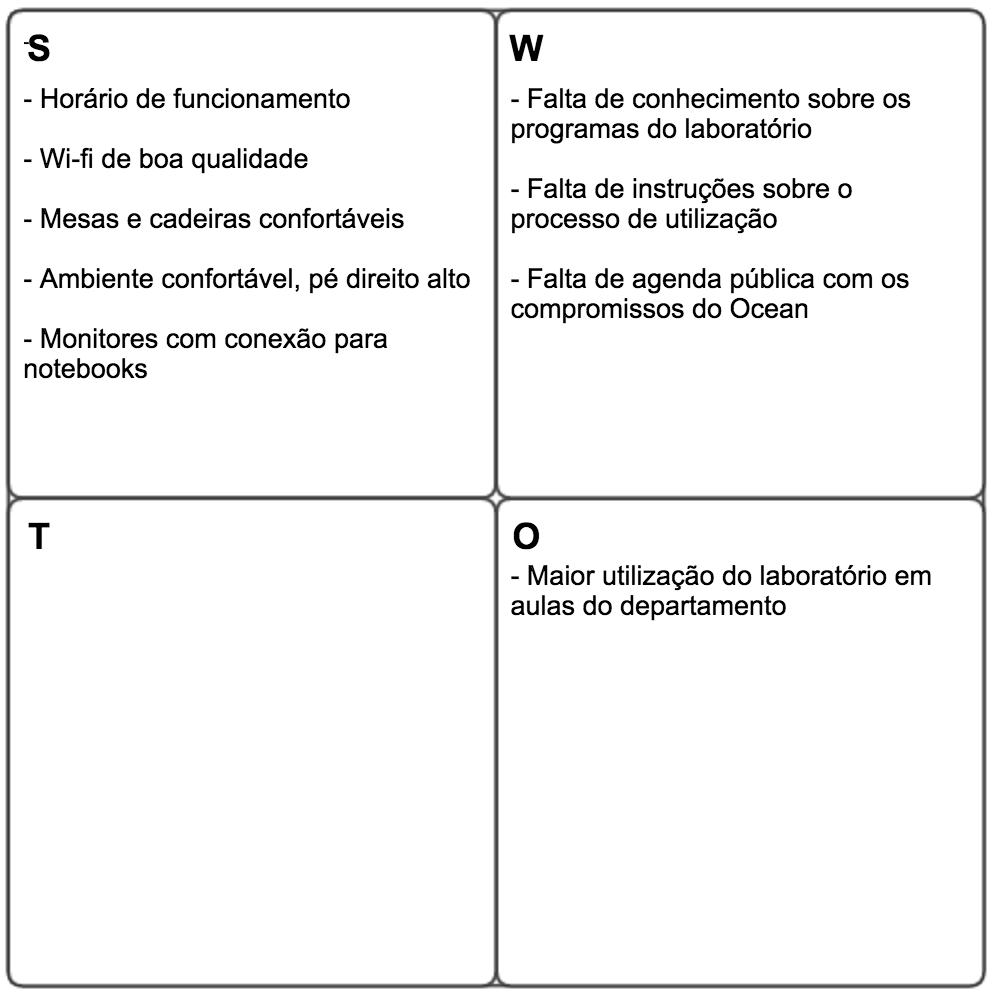
\includegraphics[scale=0.75]{img/alunosswot}}
\label{fig:swotalunos}
\caption* {Fonte: Elaborado pelo próprio autor}
\end{figure}

\section{Cursistas}

A análise dos cursistas é segmentada devido aos dois tipos de cursos dados pelo laboratório e o tipo de material a ser analisado para cada. Para os alunos de cursos básicos, foi utilizada a metodologia de \citeonline{bardin} para analisar os questionários de respostas, ao passo que com os alunos de cursos intensivos foram realizadas entrevistas semi-estruturadas.

\subsection{Cursos Básicos}

Em relação aos cursistas dos cursos básicos, utilizamos o software desenvolvido pelo autor para mapear as palavras com maior recorrência nas respostas dos questionários para cursos básicos, para as seguintes perguntas:

\begin{itemize}
\item O que mais o motivou nesse curso?
\item O que você acha que pode ser melhorado?
\item Qual tema você gostaria que fosse abordado num próximo curso?
\end{itemize}

Como forma de simplificação, foram utilizados como nomenclatura de cada questão os termos 'motivação', 'melhorias' e 'novidades', respectivamente. Em seguida, foi aplicada a metodologia de \citeonline{bardin} para as respostas de cada uma.

\subsubsection*{Pré-exploração do material}

A pré-exploração segue o mesmo modelo para todas as questões, devido aos seguintes motivos:

\begin{description}
\item[Modelo único de coleta] O instrumento de coleta de dados utilizado nas pesquisas foi o mesmo questionário reutilizado nos últimos 2 anos. Dado que no momento de preenchimento os cursistas acabaram de realizar os cursos, a percepção deles diante do conteúdo passado está bem fresca, e a contribuição também acaba sendo maior com uma taxa maior de respostas. Isso permitiu que o autor minimizasse a possibilidade de encontrar poucos dados ou dados inconsistentes com a realidade apresentada no curso.
\item[Perguntas sequenciais com o mesmo formato] As perguntas qualitativas no final do questionário são bastante diretas e fáceis de serem respondidas. O objetivo de cada questão pode ser traduzido pela própria nomenclatura previamente estabelecida: identificar a motivação dos cursistas que optaram por 'gastar' cerca de 3 horas em um curso de capacitação, identificar melhorias dentro do próprio curso para melhorar a sua qualidade de forma geral, e estar sempre atualizado para identificar a sinergia entre esse curso e outros temas de interesse dos cursistas. O formato das perguntas permitiu uma análise não exaustiva de dados pois as respostas apresentavam algumas poucas linhas, e a informação presente é suficiente para atender as necessidades da Samsung.
\item[Respostas consolidadas em um mesmo lugar] Todas as respostas foram consolidadas em planilhas digitais, de tal forma que cada resposta corresponde a uma linha, e cada pergunta é uma coluna. Esse formato simplificou a leitura flutuante realizada sobre as respostas, pois um simples \textit{scroll} na tela já traz um novo set de respostas, sem haver muito desgaste mental do autor.
\end{description}

Conforme foi ressaltado, a leitura flutuante foi o principal elemento da pré-exploração do material, pois permitiu identificar o tamanho das respostas (curtas), a variedade das respostas (baixa) e a consequente pré-aprovação da possibilidade de analisá-las e categorizá-las posteriormente. Embora sejam só características relativas observas pelo autor, elas representam a inferência ilustrada por \citeonline{bardin} como pontos de partida ou hipóteses para as próximas etapas.

\subsubsection*{Definição das unidades de análise}

Embora o autor já tivesse ideia da convergência das respostas para certos temas devido às observações obtidas na fase de pré-exploração, não saberia ainda descrever quais seriam os temas principais, e muito menos quantificá-los por número de incidências. Portanto, de forma a tentar atribuir as principais categorias, foi decidido analisar o número de incidências de cada palavra em todas as respostas, por se tratarem de textos curtos e informais.

Após uma análise inicial, observou-se que muitas palavras tinham sinergia entre si e apresentavam-se dentro de um mesmo contexto. Portanto também foram mapeadas todas as palavras que aparecem em uma mesma frase que outro palavra. Dessa forma é possível observar as palavras que aparecem em um mesmo contexto, e logo, possuem bastante sinergia entre si.

Foi considerado como premissa que todas as palavras de cada resposta não se repetem na mesma resposta - com exceção de palavras auxiliares, como artigos e pronomes - de tal forma que seria possível atribuir a linha de origem de cada palavra sem repetições.

\subsubsection*{Tratamento dos dados}

De forma a configurar o software a trabalhar em cima das respostas, foi feita uma extração dos dados da planilha no software \textit{Numbers} em um MacBook para o formato CSV, que é um arquivo de texto puro com quebras de linha e separação por vírgulas. Como o arquivo original, cada linha corresponde a uma resposta e cada elemento entre vírgulas corresponde a uma pergunta. Portanto para cada pergunta a ser analisada, são percorridas todas as linhas e só analisados os elementos correspondentes.

Por se tratarem de todas as palavras da língua portuguesa, foi feito um trabalho manual e iterativo de descartar todas as palavras que não agregariam valor semântico esperado à frase, como pronomes, artigos, verbos auxiliares, conjunções e preposições. Foi uma opção não realizar uma integração com algum software ou \textit{Web API} de Língua Portuguesa pela necessidade e esforço em garantir a confiabilidade do mesmo, portanto a partir do próprio conhecimento do idioma foram feitas iterações e remoções de palavras indesejadas.

Também foram eliminadas as palavras relativas à 'curso' e 'aula', pois todas as perguntas são direcionadas a como melhorar, motivar ou trazer novas coisas para o curso e para a aula, portanto foram consideradas redundantes para a análise.

Outro tratamento realizado foi a remoção de espaços em excesso, pontuações e o emprego das aspas, pois estes atrapalhavam a contagem de palavras.

A partir dos tratamentos descritos e de outros específicos a cada questão, foi possível elaborar uma tabela como \textit{output} do software utilizado. A tabela representa uma contagem das principais palavras presentes nas respostas, acompanhadas de outras que aparecem em um mesmo contexto, e de um exemplo de respostas para ilustrar o uso das palavras de forma conjunta. O exemplo é obtido randomicamente através de uma busca por respostas que apresentem ambas as palavras. Para isso, foram adotadas algumas constantes para aplicação no software:

\begin{itemize}
\item Número mínimo de incidências para ser considerado na tabela: 1\% do número de respostas
\item Número de palavras com sinergia que são exibidas: 3
\end{itemize}

Esses números foram definidos posteriormente, pois foram feitos alguns testes para identificar até onde poderia ser filtrado os dados para não perder nenhuma informação relevante. Essas constantes se apresentaram boas tanto de forma ilustrativa para o trabalho quanto para a categorização posteriormente feita das palavras.

\subsubsection*{1\textsuperscript{a} Questão: \textit{Motivação} - Tratamento dos dados }

Novamente, como não há integração com um dicionário de Língua Portuguesa, foi possível de fazer agrupamentos de palavras qeu se encontravam em um mesmo contexto, comprovado pelas sinergia com as mesmas palavras ou similares. 

Foi possível agrupar posteriormente palavras que se apresentavam em diferentes flexões gramaticais de número, como: 

\begin{itemize}
\item 'conhecimento' e 'conhecimentos'
\item 'tecnologia' e 'tecnologias' 
\item 'novas' e 'nova' 
\item 'ferramenta' e 'ferramentas' 
\item 'novos' e 'novo' 
\item 'apps' e 'app'
\item 'aplicativos' e 'aplicativo'
\end{itemize}

Também foram agrupadas palavras com flexões gramaticais de gênero:

\begin{itemize}
\item 'novas' e 'novos'
\end{itemize}

Por fim, palavras com mesmo nível semântico:

\begin{itemize}
\item 'app' e 'aplicativo'
\item 'instrutor' e 'professor'
\end{itemize}

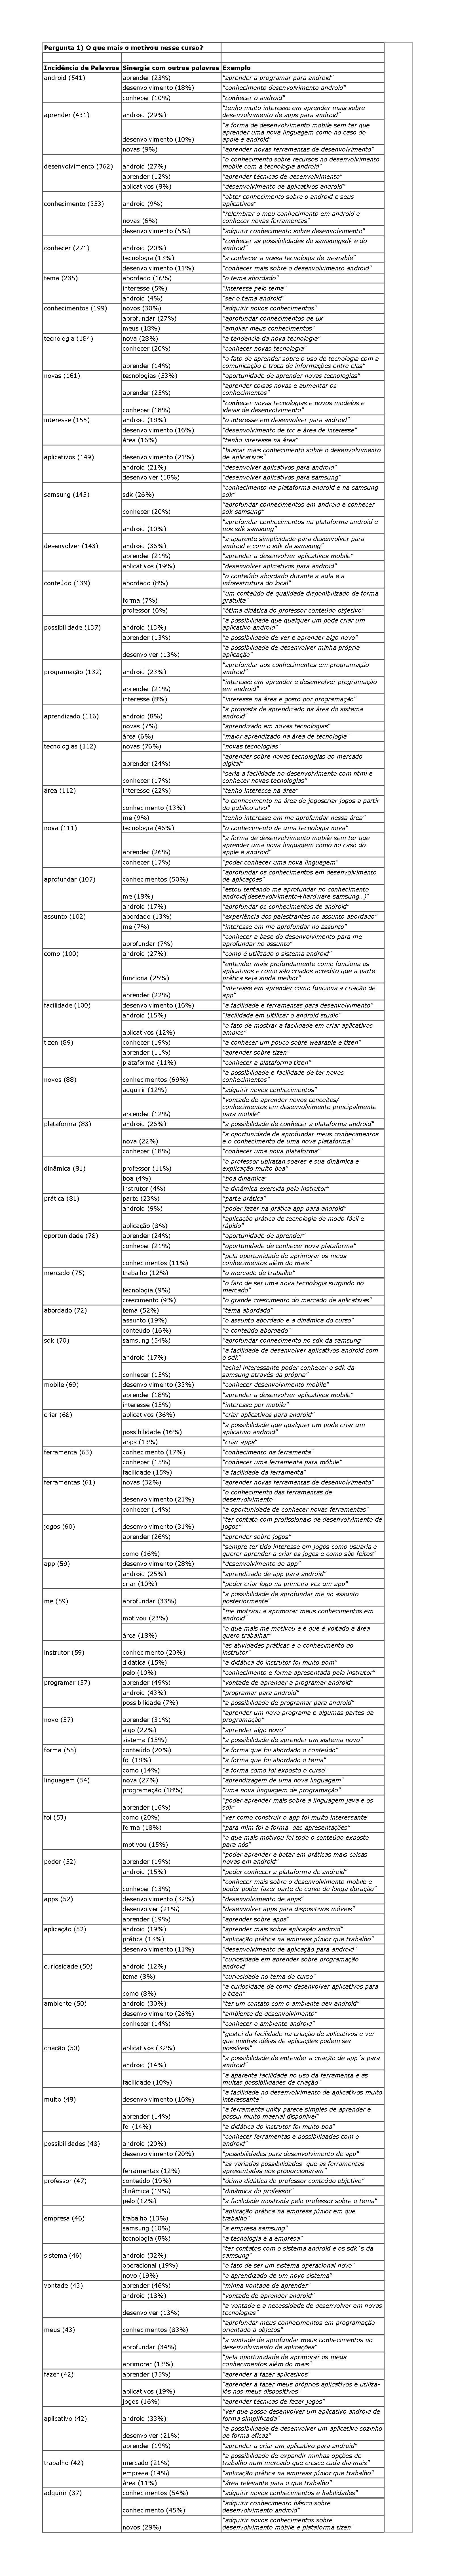
\includepdf[pages=-, pagecommand={}]{Pergunta1.pdf}

\subsubsection*{1\textsuperscript{a} Questão: \textit{Motivação} - Categorização e sub-categorização }

Após analisar a incidência de palavras, foi possível observar a partir dos exemplos uma ambiguidade promovidos pela pergunta em questão. A interpretação correta dessa pergunta seria "quais foram os pontos do curso que você achou mais interessante / relevante?", porém a maior parte das respostas aparentemente a interpretou como "o que o motivou a fazer o curso?". Isso gerou uma séria de respostas relacionadas ao próprio tema do curso, como "interesse por desenvolvimento android e SDK da samsung". Dado que o tem mais recorrente de apresentação do curso chama-se "Introdução ao Desenvolvimento de Aplicativos Android \& Samsung SDK", acaba-se por ter respostas redundantes. Também ocorreram respostas inerentes ao contexto de mercado de trabalho envolvendo programação, o que também foge do objetivo proposto por essa pergunta. Foi passado para a Samsung uma proposta de reformulação dessa pergunta, baseada em como deseja-se utilizar essa informação posteriormente.

Entretanto, ainda foi possível extrair algumas informações a respeito de pontos elogiados do curso, como:

\begin{itemize}
\item A ocorrência de 'professor' e 'dinâmica' indicaram a aceitação pelos alunos do modelo proposto pelo curso, e elencaram estes como um fator motivador.
\item A palavra 'prática' indica que os alunos gostaram da parte prática dos cursos, que indiretamente deve contribuir com a dinâmica elogiada no item anterior.
\end{itemize}

A partir desses pontos, foram extraídas as seguintes categorias para a questão "O que mais o motivou nesse curso?":

\begin{figure}[H]
\caption{Categorias para a questão 1}
\centerline{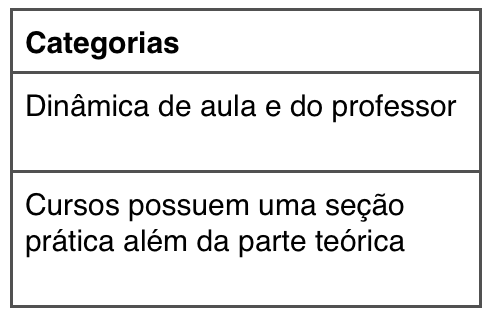
\includegraphics[scale=0.75]{img/categoriasmotivacao}}
\label{fig:categoriasmotivacao}
\caption* {Fonte: Elaborado pelo próprio autor}
\end{figure}

\pagebreak
\subsubsection*{2\textsuperscript{a} Questão: \textit{Melhorias} - Tratamento dos dados }

Em relação à flexão gramatical de número e gênero e semântica, foram agrupadas as seguintes palavras

\begin{itemize}
\item 'práticas', 'práticos', 'prático' e 'prática'
\item 'professor', 'instrutor', 'instrutores' e 'professores'
\item 'conhecimento' e 'conhecimentos'
\item 'app', 'apps', 'aplicativo' e 'aplicativos'
\end{itemize}

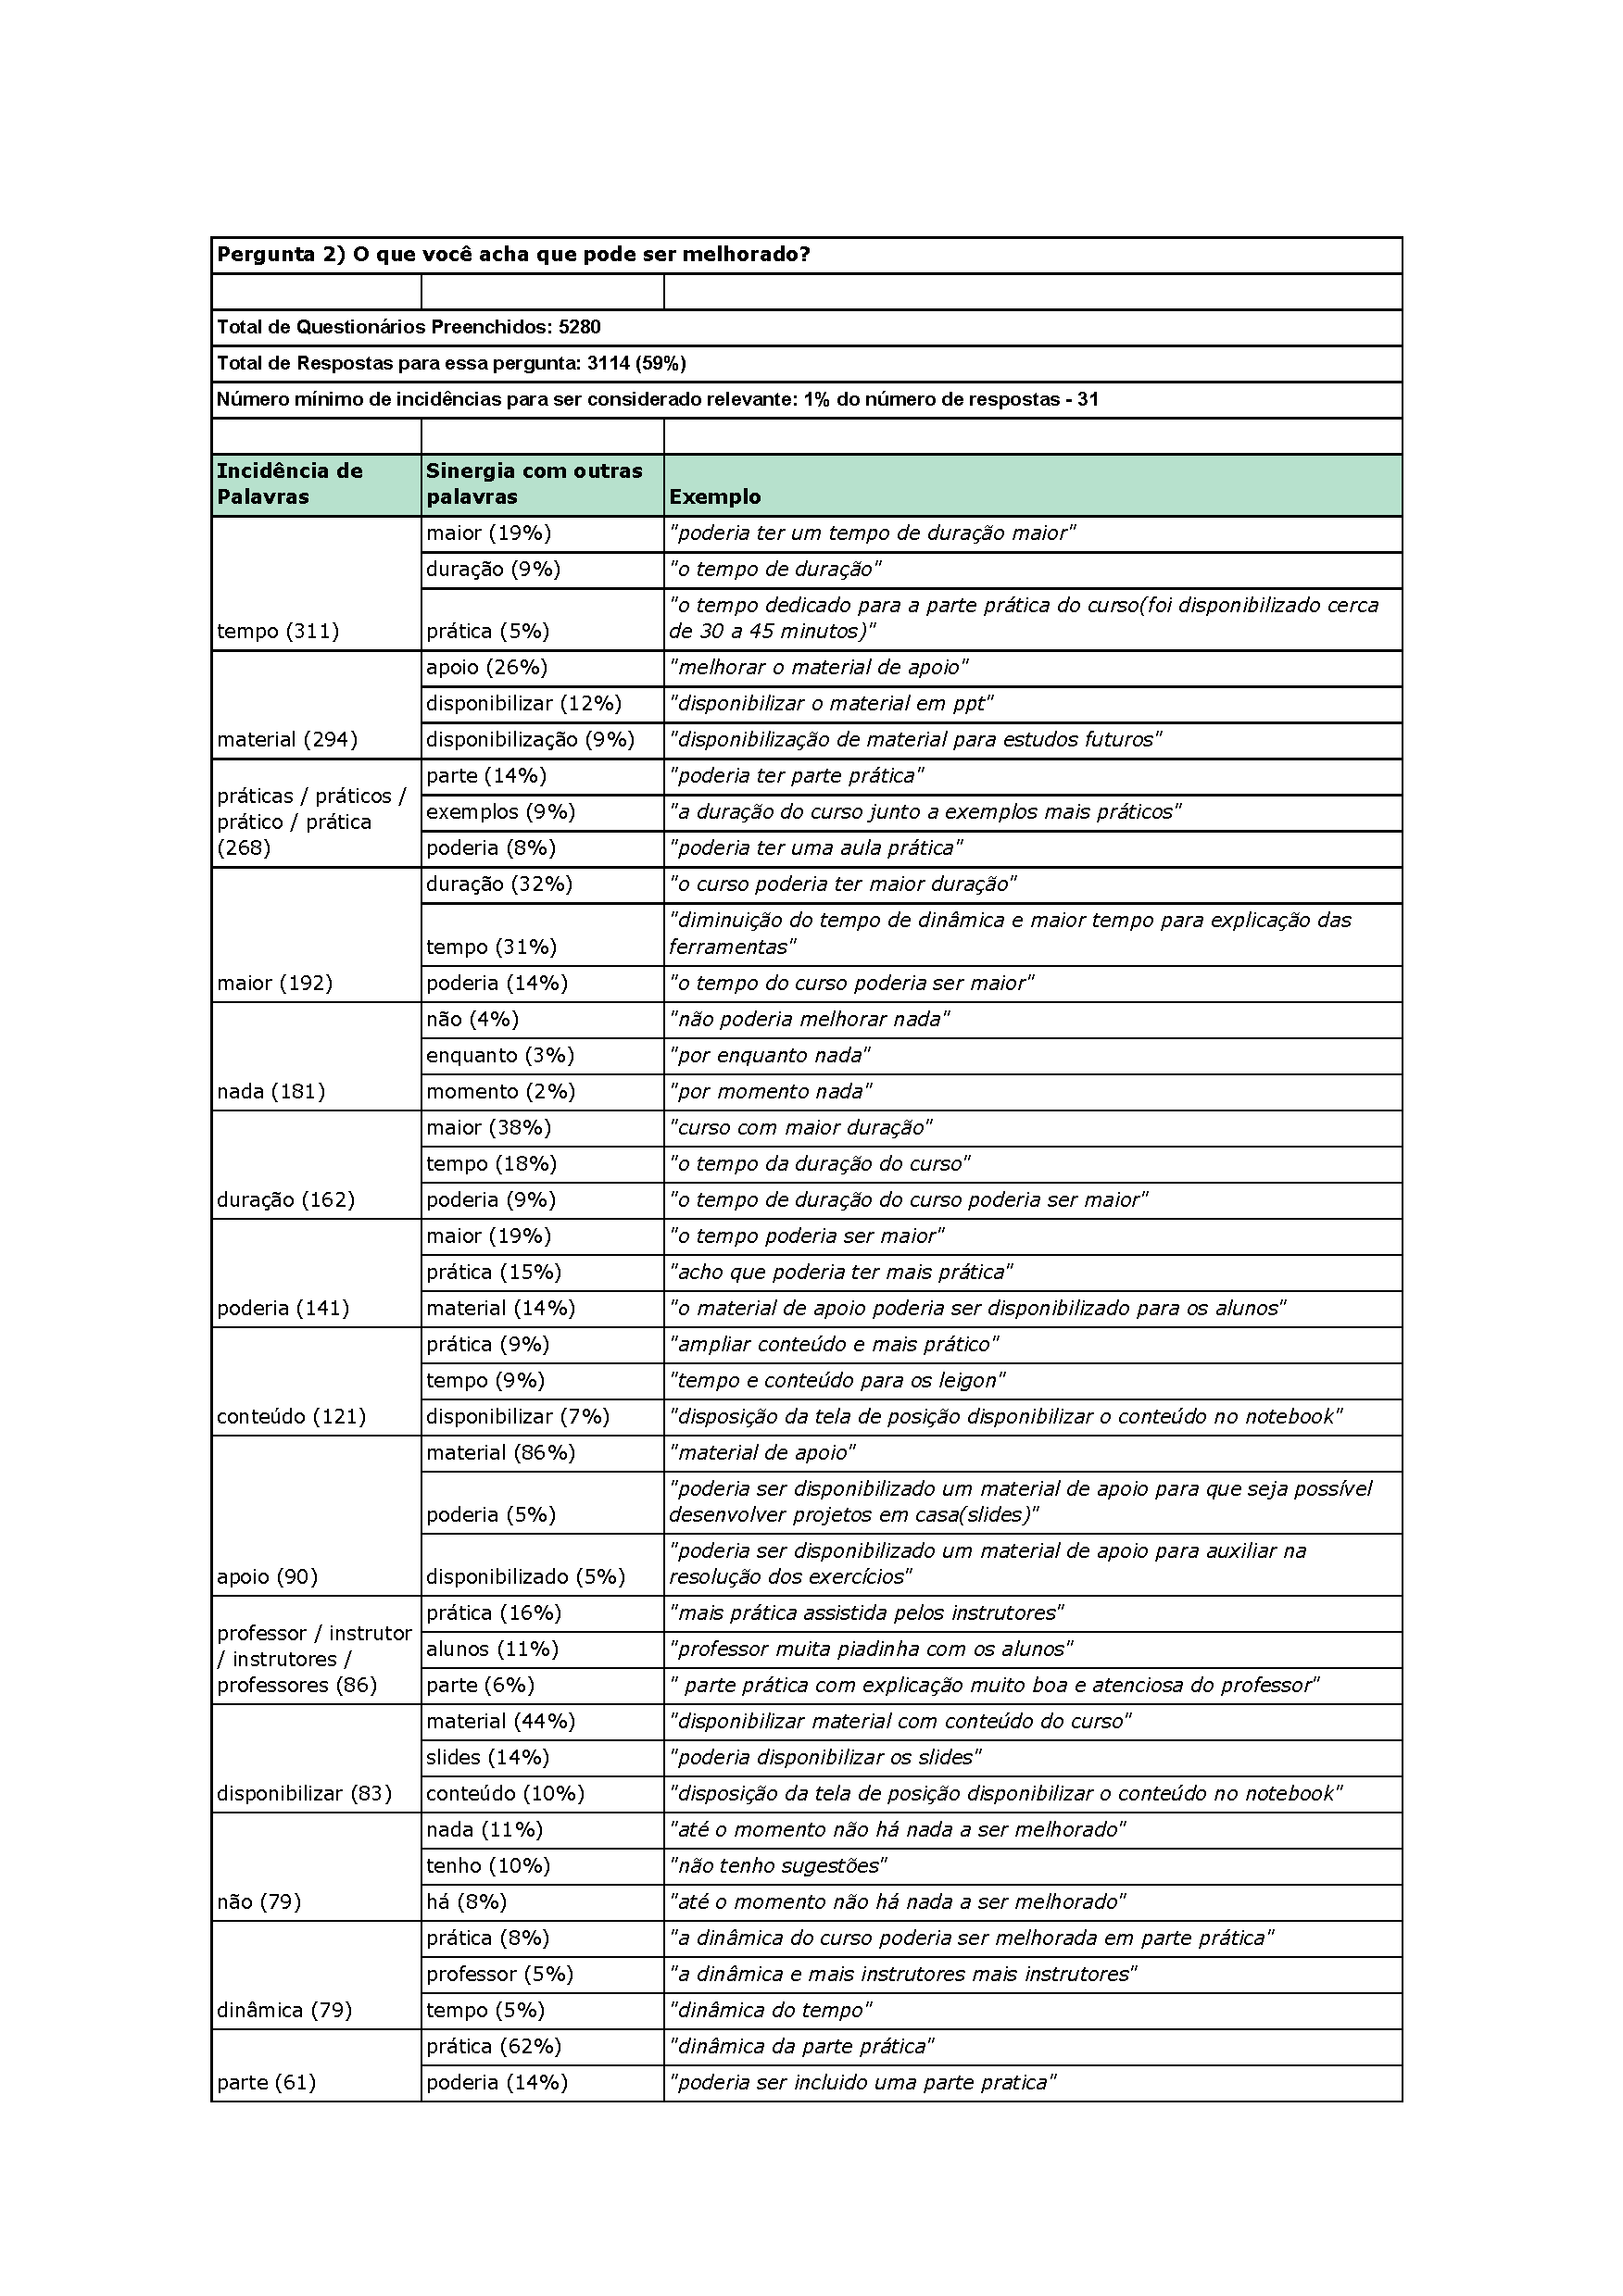
\includepdf[pages=-, pagecommand={}]{Pergunta2.pdf}

\subsubsection*{2\textsuperscript{a} Questão: \textit{Melhorias} - Categorização e sub-categorização }

Diferentemente da questão anterior, esse item é compreendido muito melhor pelos alunos, e as respostas tornam-se muito mais objetivas. A recorrência já mostra de imediato três pontos a serem melhorados, a duração do curso, problemas com o material de apoio e a inclusão de mais modalidades práticas dentro da aula. Esses problemas, de forma conjunta, correspondem a cerca de 40\% das respostas analisadas.

A duração do curso se mostra um grande problema, se mostrando incidente através das palavras 'tempo', 'duração' e 'carga horária', essa última com as duas palavras aparecendo na tabela.

Os problemas com o material de apoio também se mostra recorrente através da expressão 'material de apoio', 'conteúdo', 'slides', 'slides' e 'apresentação'. A maior parte se associa com as palavras 'disponibilizar' e 'disponibilização', indicando que o material utilizado não é entregue para os alunos.

A recorrência de termos ligados à prática indica que há uma necessidade de aumentar a parte prática no programa diante da teórica. Aliada essa informação à questão da carga horária, deve ser desejável que se for possível aumentar o tempo de curso, que ele aumenta em termos práticos e não teóricos.

Em menor volume (menos de 5\% cada), aparecem questões como maior flexibilização do horário ou disponibilidade de horários, através das palavra 'horário' e 'dias', e problemas com equipamentos no laboratório.

A partir desses pontos, foram extraídas as seguintes categorias para a questão "O que você acha que pode ser melhorado?":

\begin{figure}[H]
\caption{Categorias para a questão 2}
\centerline{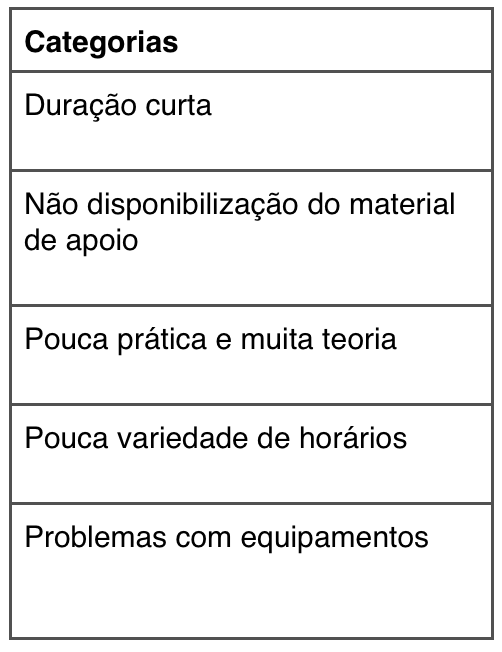
\includegraphics[scale=0.75]{img/categoriasmelhorias}}
\label{fig:categoriasmelhorias}
\caption* {Fonte: Elaborado pelo próprio autor}
\end{figure}

\subsubsection*{3\textsuperscript{a} Questão: \textit{Novidades} - Tratamento dos dados }

Em relação à flexão gramatical de número e gênero e semântica, foram agrupadas as seguintes palavras

\begin{itemize}
\item 'jogos', 'jogo', 'game' e 'games'
\item 'aprofundar' e 'aprofundamento'
\item 'práticas', 'práticos', 'prático' e 'prática'
\item 'app', 'apps', 'aplicativo' e 'aplicativos'
\end{itemize}

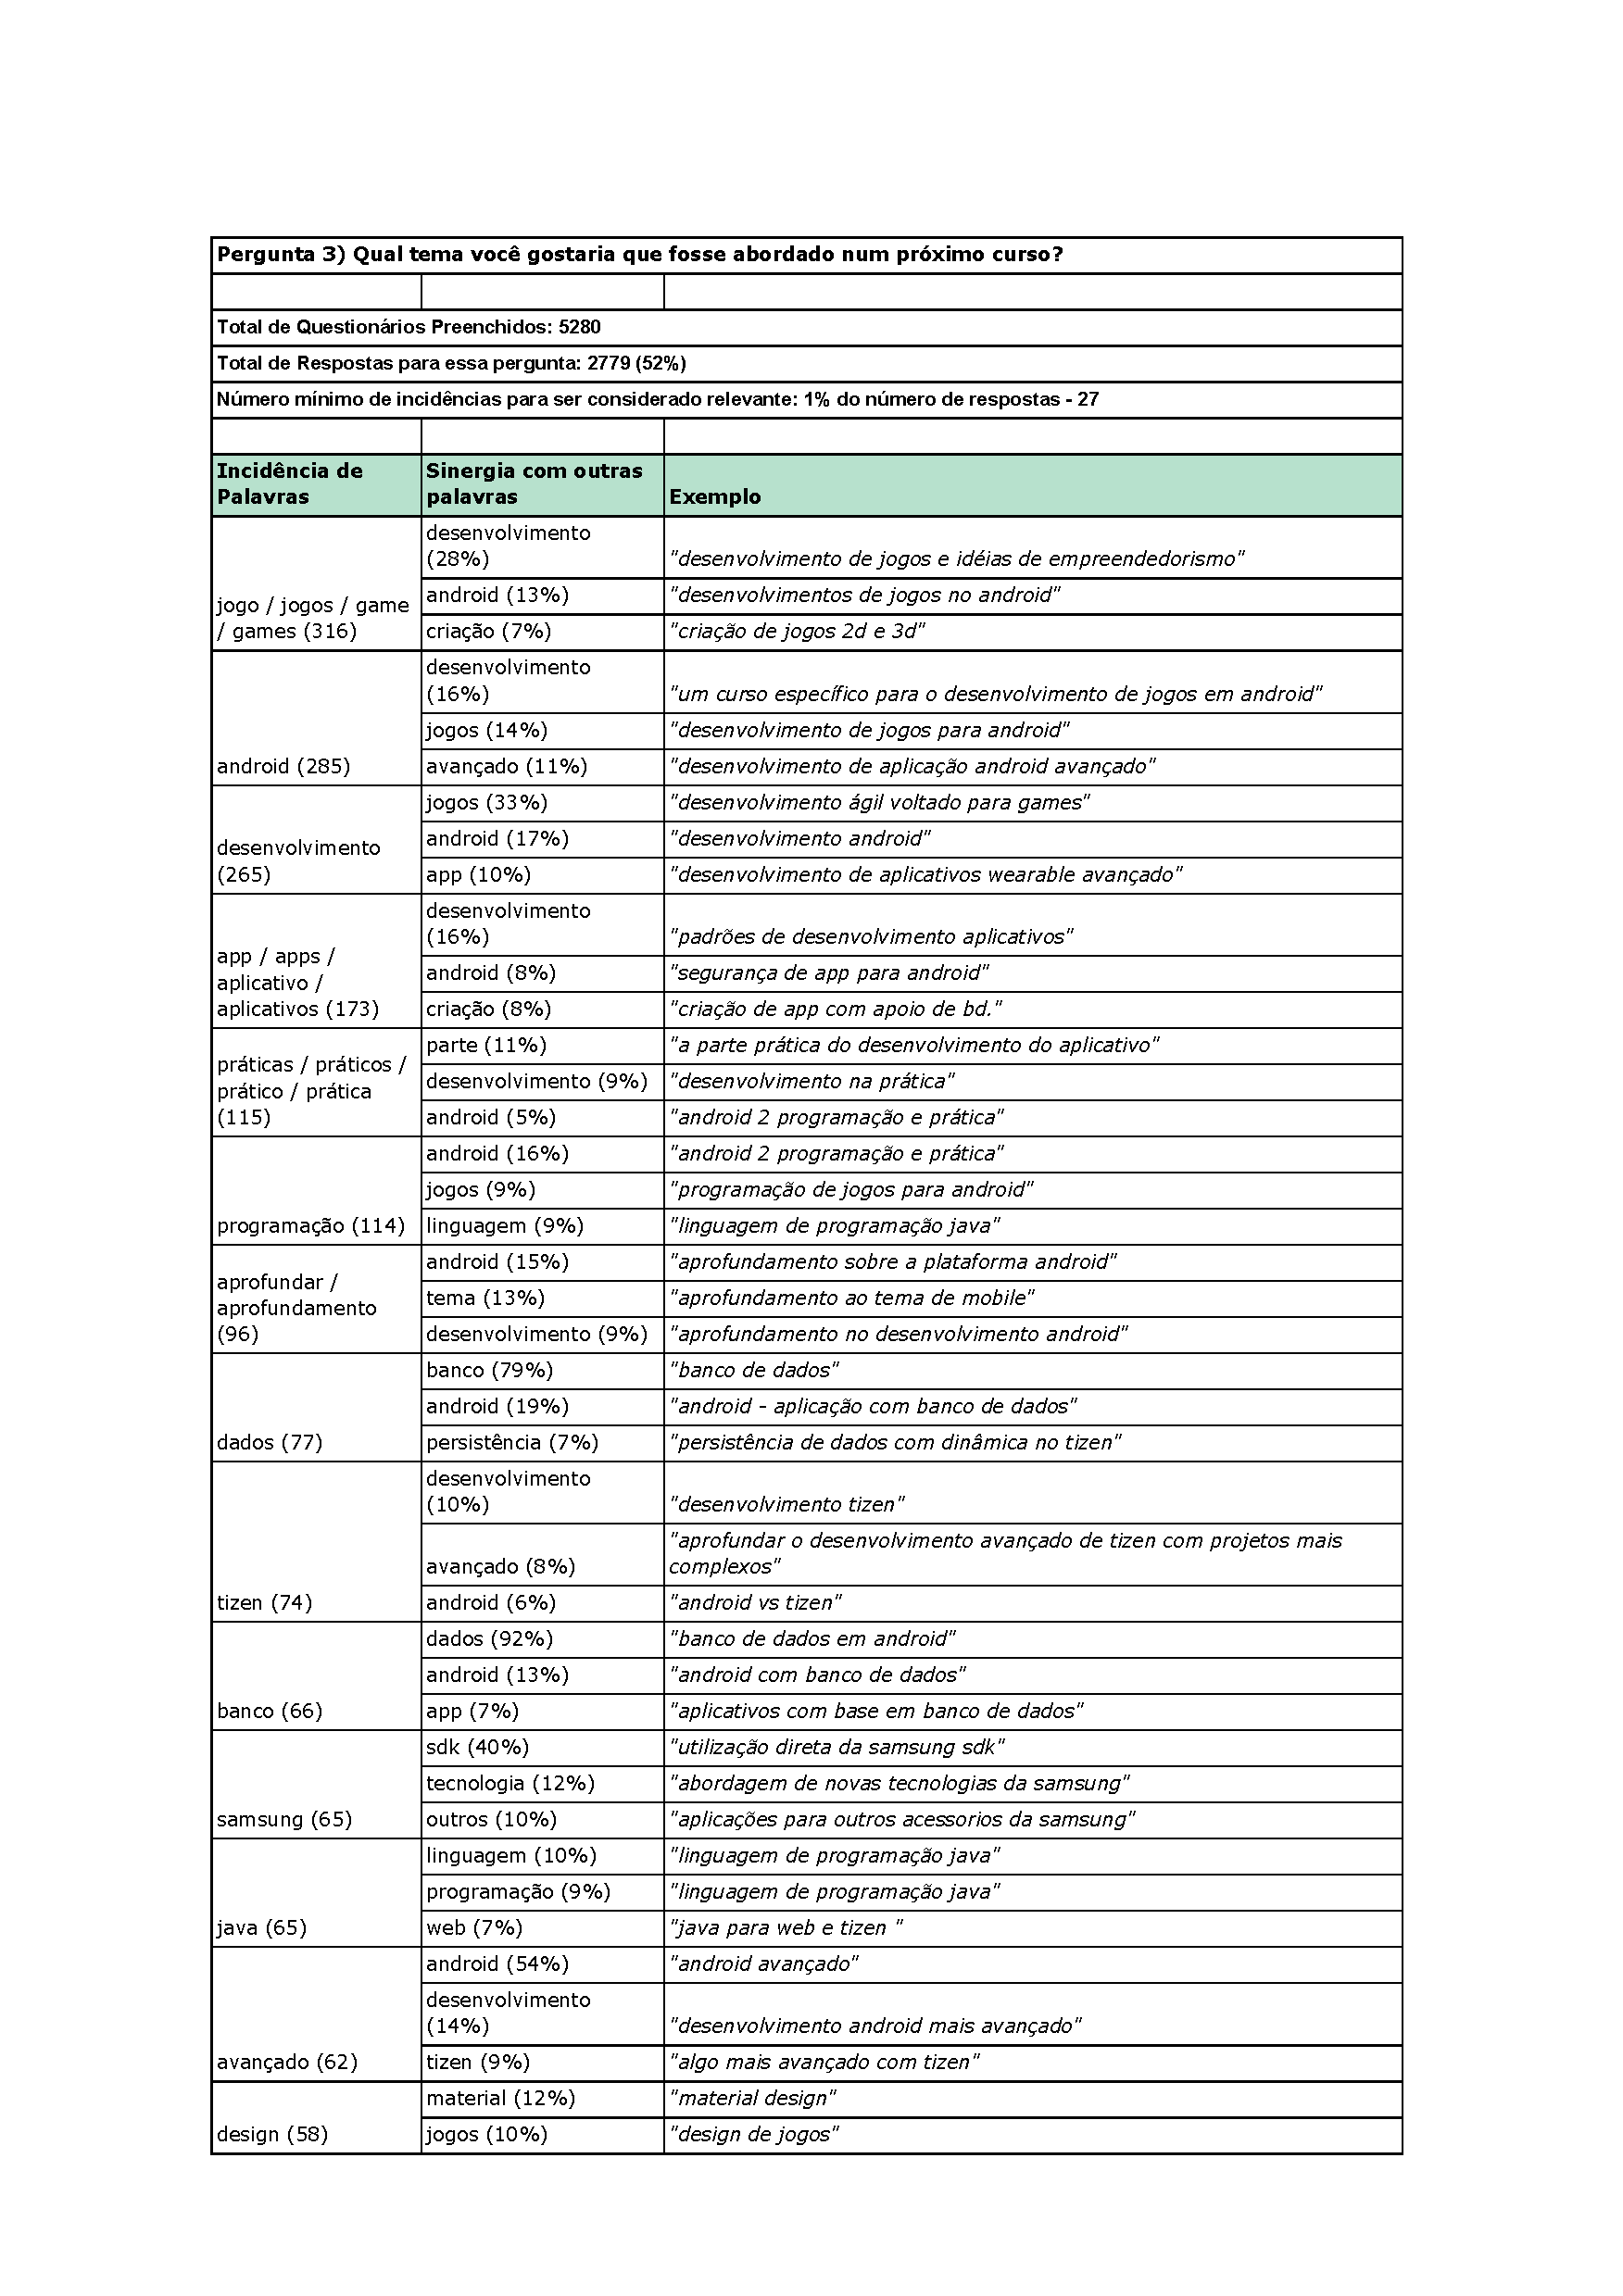
\includepdf[pages=-, pagecommand={}]{Pergunta3.pdf}

\subsubsection*{3\textsuperscript{a} Questão: \textit{Novidades} - Categorização e sub-categorização }

Em primeira instância, é possível visualizar uma grande demanda de alunos por aulas específicas para o desenvolvimento de jogos. É de grande relevância que esta questão é a de escopo mais aberto das três, portanto a grande recorrência do termo 'jogo' nesse contexto é bastante relevante. Além de jogos, existe uma demanda pela aplicação de android em outros casos de uso, como aplicativos ou uma exploração mais avançada do sistema operacional. 

Em menor volume porém com uma maior gama de opções, existe uma demanda por uma exploração de bancos de dados, tizen, maior exploração do sdk da samsung e outras tecnologias, linguagem de desenvolvimento java, design e user experience, desenvolvimento web, web services, e unity. 

A partir desses pontos, foram extraídas as seguintes categorias para a questão "Qual tema você gostaria que fosse abordado num próximo curso?" :

\begin{figure}[H]
\caption{Categorias para a questão 3}
\centerline{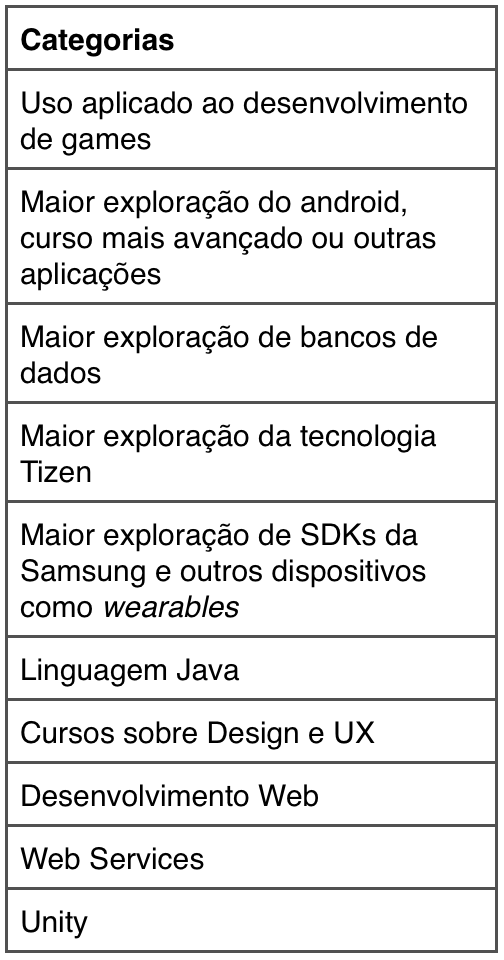
\includegraphics[scale=0.75]{img/categoriasnovidades}}
\label{fig:categoriasnovidades}
\caption* {Fonte: Elaborado pelo próprio autor}
\end{figure}

A partir das categorias obtidas para todas as questões, foi definida a seguinte análise:

\begin{figure}[h]
\caption{Análise do Ocean - Cursistas - Cursos Básicos}
\centerline{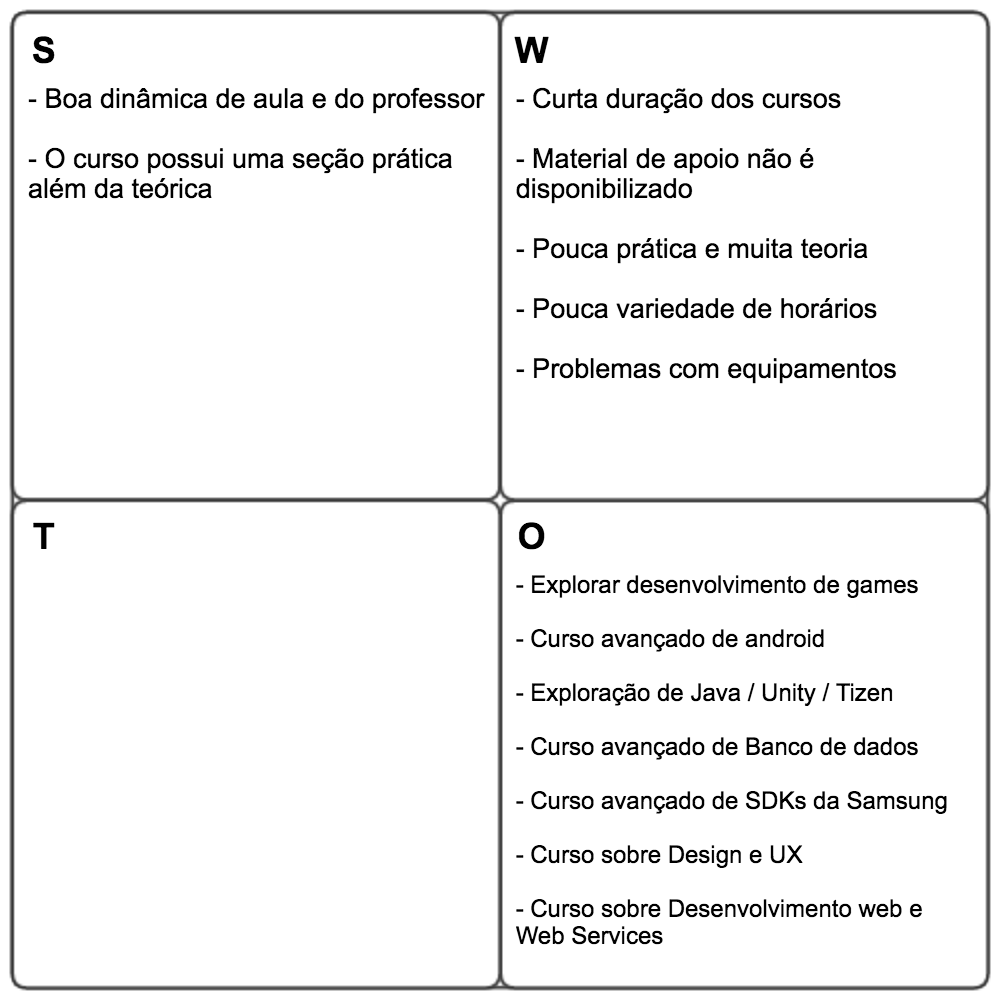
\includegraphics[scale=0.75]{img/cursosbasicosswot}}
\label{fig:swotcursosbasicos}
\caption* {Fonte: Elaborado pelo próprio autor}
\end{figure}

\subsection{Cursos Intensivos}

Para a análise dos cursos intensivos, foram feitas entrevistas com os grupos participantes da edição atual do módulo de pré-aceleração do programa Ocean. As entrevistas foram realizadas em um dia de mentoria, considerado mais tranquilo para a conversa com todos os grupos presentes.

As conversas com os cursistas foram muito produtivas e os mesmos foram extremamente atenciosos, em primeira instância pois já tinham sido avisados das entrevistas naquele dia, e também porque eles têm bastante orgulho das suas ideias e gostam muito de falar sobre elas e receber \textit{feedbacks}. Essas conversas foram bastante apreciadas pelo autor pois foi importante para quebrar alguns conceitos que subconscientemente já tinha estabelecido:

\begin{description}
\item[Os cursistas serão alunos de graduação ou recém-formados] 

Embora alguns grupos fossem de alunos em graduação ou com graduação há menos de 2 anos, alguns grupos era constituídos de pessoas com bastante experiência no mercado de trabalho, incluindo um grupo que o líder é um senhor com mais de 40 anos de experiência em gestão de empresas. Também há alunos de mestrado e pessoas com mais experência com \textit{startups} e as novas tecnologias.

\item[Os cursistas dedicam-se ao projeto em paralelo a um emprego fixo] 

Muitas das pessoas que participam do programa estão se dedicando praticamente todo tempo delas para esse projeto, abrindo mão dos antigos empregos para focar completamente nele. Em especial um casal de Brasília vem para São Paulo e volta toda semana para acompanhar as aulas do curso. Segundo eles todo esforço vai valer a pena para poderem lançar o produto deles, de cunho sócio-ambiental, e a gratuidade do programa já compensa pelo que pagariam por um curso de mesma qualidade em Brasília.

\end{description}

Em comum a todos os grupos, foi possível observar a vontade que eles têm de fazer o produto ser bem-sucedido e a atenção com que escutam e recebem os \textit{feedbacks} dos mentores. O reflexo dessa dedicação se dá na avaliação positiva em relação à intensidade do curso e aos modelos de \textit{checkpoint} semanais realizados pelo programa, que consideram "puxada" porém necessária para forçar o grupo a ter agilidade em relação a mudanças e obtenção de respostas em relação ao produto. Não obstante, ainda mostra que o programa Ocean realmente está comprometido com os projetos a serem acelerados.

De acordo com o cronograma do programa Ocean, os grupos só trabalharam até o momento a parte de \textit{Customer Discovery}, entretanto todos ficaram muito satisfeitos com essa primeira parte do curso, exaltando a excelente qualidade do trabalho da aceleradora Baita. A qualidade dos executivos da Baita foi ressaltada inclusive pelo senhor mais experiente dos grupos, que considerou como os melhores professores / mentores que já teve, mesmo participando de programas de aceleração pagos.

Mesmo com grande satisfação dos cursistas, algumas questões foram levantadas, como a ineficiência de palestras de 3 horas, pois consideram que esse tipo de modalidade é apenas uma transmissão de conhecimento, ao passo que o mesmo palestrante poderia conversar com os grupos e o aprendizado poderia ser mais direcionado. Também foi ressaltado que havia uma diferença considerável entre o estado de maturidade dos produtos de cada grupo, o que atrapalhava um pouco a \textit{gamificação} proposta pelo programa, em que os grupos deveriam competir pelo número de entrevistas a serem realizadas com o público-alvo. Muitas vezes essa \textit{gamificação} também era atrapalhada pela diferença natural do modelo de negócio entre produtos, pois um produto B2B é mais difícil de conseguir entrevistas do que com produtos B2C.

Por fim, acredita-se que a Samsung poderia explorar mais a questão de inovações e tendências tecnológicas para inspirar os cursistas a melhorar a tecnologia de seus produtos. Houveram palestras relacionadas ao tema, porém aparentemente elas rodaram muito em torno de produtos da empresa de forma não natural, fazendo com que parecesse que fosse uma propaganda direta dos produtos. A mesma informação poderia ser passada ao explorar os problemas reais enfrentados pelos usuários e pelo mercado e aí sim mostrar como a Samsung criou soluções para esses problemas.

A partir das conversas com os cursistas, foi obtida a seguinte análise:

\begin{figure}[h]
\caption{Análise do Ocean - Cursistas - Cursos Intensivos}
\centerline{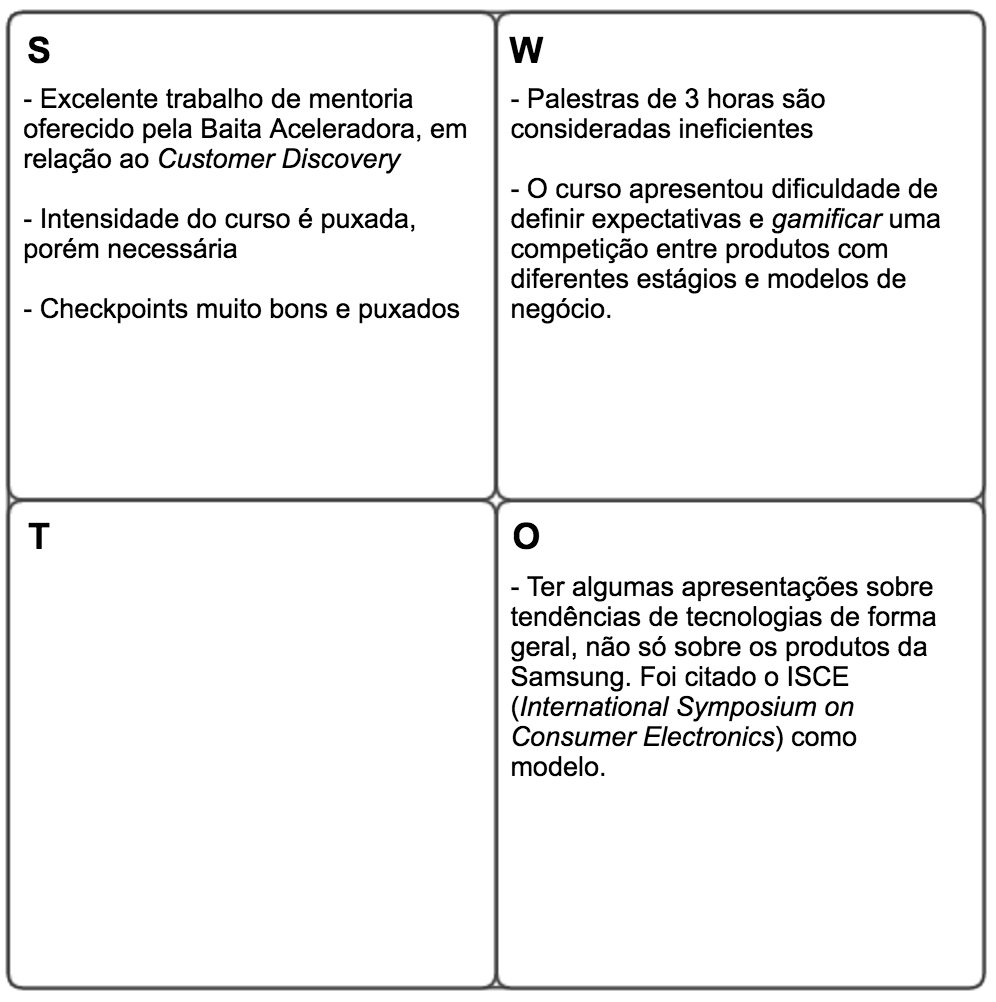
\includegraphics[scale=0.75]{img/cursosintensivosswot}}
\label{fig:swotcursistasintensivos}
\caption* {Fonte: Elaborado pelo próprio autor}
\end{figure}

\chapter{Propostas}
\label{cha:propostas}

Esse capítulo tem como base os elementos de desenvolvimento do programa Ocean levantados no capítulo anterior, e tem como objetivo definir e criar uma proposta de desenvolvimento para um deles. Embora todos os pontos sejam levados até a gestão PRO/Samsung, somente um deles será desenvolvido de forma a ser o suficiente para ilustrar o trabalho sem ultrapassar o seu propósito acadêmico.

\section{Definição do elemento de desenvolvimento}

Em conjunto com o PRO e a Samsung, foi realizada uma triagem dos pontos a serem desenvolvidos, através de algumas etapas de exclusão e posteriormente de seleção do ponto a ser trabalhado.

\begin{description}
\item[Exclusão dos pontos levantados pelos cursistas] - Em relação aos pontos levantados sobre \textit{feedbacks} dos cursistas, será elaborado um relatório executivo com menor teor acadêmico porém mais detalhes diante das análises realizadas. Em relação aos cursos básicos, poderá será feita uma segmentação dos \textit{feedbacks} por ano de realização do questionário ou por tipo de curso dado pelo laboratório. Já para os cursos intensivos, poderão explorados os pontos levantados do ponto de vista de cada grupo, incluindo a identificação de 'frases de efeito' que poderiam ser utilizadas em um material de divulgação do curso. Não obstante, como esses pontos devem ser trabalhados quase que exclusivamente pela gestão da Samsung, serão levantadas questões a respeito de como desenvolver esses pontos, porém eles serão excluídos dentro do contexto desse trabalho.

\item[Exclusão de pontos considerados "passivos"] - Alguns pontos levantados não geram nenhuma ação a ser realizada por parte da gestão do laboratório, pois a gestão já permite o seu desenvolvimento, só faltando oportunidades ou resultados que aparecerão com o tempo. Entre esses pontos estão "Utilização do laboratório para a pós-graduação, na geração de pesquisas", "Maior utilização do laboratório em aulas do departamento", "Expansão dos projetos e parcerias (NEU) além dos cursos intensivos" e "Instituições de aceleração de empresas não-gratuitas podem tentar entrar na universidade". Os três primeiros pontos não apresentam nenhuma barreira para se desenvolverem naturalmente, e são fatores que a gestão acompanhará de perto. O último é considerado pela gestão improvável de acontecer pois com o aumento de instituições de aceleração oferecendo cursos bons gratuitos dentro da universidade, as instituições pagas têm menos incentivo para querer entrar na universidade.

\item[Exclusão de pontos considerados operacionais] - Os pontos operacionais são aqueles que podem ser corrigidos com alguma ação a ser tomada sem a necessidade de tomar algum decisão considerada estratégica pela gestão. Dentro desses pontos estão "Falta de conhecimento sobre os programas do laboratório", "Falta de instruções sobre o processo de utilização" e "Falta de agenda pública com os compromissos do Ocean". São pontos relevantes, e a gestão deverá fazer algo a respeito deles para maximizar o uso do laboratório pelos alunos.

\end{description}

Após a triagem inicial, restaram-se os seguintes pontos:

\begin{table}[h]
\caption{Elementos de desenvolvimento}
\centerline{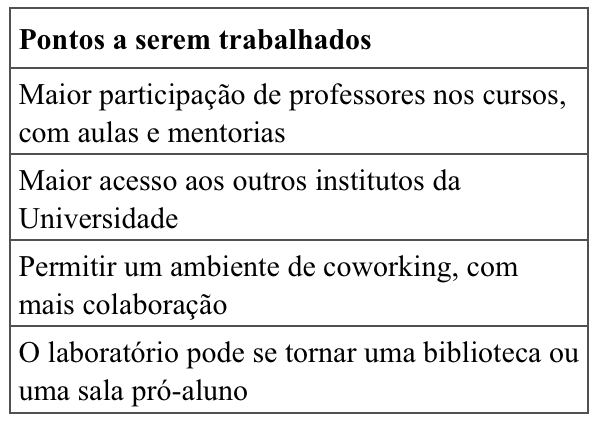
\includegraphics[scale=0.75]{img/pontosselecionados}}
\label{fig:pontosselecionados}
\caption* {Fonte: Elaborado pelo próprio autor}
\end{table}

Os dois primeiros pontos em questão estão sendo avaliados pelo departamento, pois envolvem uma remuneração extra para os professores participarem nesses cursos e uma maior divulgação do laboratório por parte de todos os \textit{stakeholders}, principalmente o NEU e o PRO. Portanto juntamente à gestão do PRO e da Samsung, foi definido que seria desenvolvido o terceiro ponto mencionado, \textbf{"Permitir um ambiente de \textit{coworking}, com mais colaboração"}, pois além de ser uma questão estratégica para o laboratório, ele pode evitar o problema de o laboratório se tornar uma biblioteca ou uma pró-aluno.

%!TEX root = index.tex
\section[Conclusão]{Conclusão}
\begin{frame}{Conclusão}
\textbf{Discussão}
\begin{itemize}
	\item Dependência entre qualidade de recomendação e $N$
	\item Mais avaliações $H$ é melhor que mais usuários $T$
	\item Muita influência de $d^f$, $\mathcal{F}$
	\item Pouca influência de $k$, $M$, $W$
\end{itemize}
\vspace{.5cm}
\textbf{Trabalhos futuros}
\begin{itemize}
	\item ``Sistema de Recomendação nas Nuvens''
	\item Eliminação de restrições de entrada/saída de dados
	\item Desenvolvimento de um \textit{driver} SQL 
	\item Reconstrução da biblioteca em C
	\item Aplicação em um banco de dados de um e-commerce real
\end{itemize}
\end{frame}

% ----------------------------------------------------------
% ELEMENTOS PÓS-TEXTUAIS
% ----------------------------------------------------------
\postextual
% ----------------------------------------------------------

% ----------------------------------------------------------
% Referências bibliográficas
% ----------------------------------------------------------
\bibliography{bibliografia}
%!TEX root = index.tex
\begin{apendicesenv}

\chapter{Questionários}

\textbf{Samsung}

\begin{enumerate}
\item Nome: Luis Guilherme Selber
\item Há quanto tempo está na Samsung?
\item Qual o seu papel em relação ao projeto Ocean?
\item Quais são os objetivos da iniciativa Ocean?
\item Quais são as modalidades de cursos que são oferecidos pelo Ocean atualmente? Quais os objetivos de cada uma?
\item O que achou da migração do Laboratório para dentro da Universidade?
\item Quais eram as expectativas em relação à operação dentro da universidade?
\item Já foram obtidos resultados em relação à essa migração?
\item Como avalia a colaboração com o departamento de engenharia de produção, em relação a - Reserva de horários; - Burocracia; - Outras interações
\item Como o Ocean realiza a divulgação de sua operação para a Universidade como um todo?
\item Como o Ocean pode expandir as suas operações?
\end{enumerate}

\clearpage

\textbf{NEU}

\begin{enumerate}
\item Nome: Juliana Uechi
\item Há quanto tempo está no NEU?
\item Quais são as propostas do NEU?
\item Quais são os projetos atuais do NEU?
\item Como funcionava o NEU antes de se sediar no PRO?
\item Como o NEU foi parar dentro do InovaLab?
\item Como é o contato do NEU com a comunidade uspiana?
\item Como o NEU avalia a contribuição do Ocean para a Universidade e para o próprio NEU?
\item Qual é a percepção do NEU de ter outra entidade com o propósito de pré-acelerar empresas dentro do PRO?
\item Quais são as interações atuais entre o NEU e o Ocean?
\item Como o NEU contribui com a divulgação do Ocean?
\end{enumerate}

\clearpage

\textbf{PRO}

\begin{enumerate}
\item Nome: Fernando Laurindo
\item Quais são os projetos que o PRO têm acompanhado de perto?
\item Qual é o interesse do PRO com o Ocean?
\item Como o Ocean se relaciona com a tríade pesquisa, ensino e extensão?
\item Como tirar mais proveito do Ocean?
\item Como o departamento vê o impacto da cultura de empreendedorismo nos alunos?
\item Acha que o Ocean cumpre bem esse papel?
\item O laboratório está atendendo as expectativas?
\item O que acha que poderia ser melhorado no laboratório?
\end{enumerate}

\clearpage

\textbf{PRO}

\begin{enumerate}
\item Nome: Eduardo Zancul
\item Quais são os projetos que o PRO têm acompanhado de perto?
\item Qual é o interesse do PRO com o Ocean?
\item Como o Ocean se relaciona com a tríade pesquisa, ensino e extensão?
\item Como tirar mais proveito do Ocean?
\item Como o departamento vê o impacto da cultura de empreendedorismo nos alunos?
\item Acha que o Ocean cumpre bem esse papel?
\item O laboratório está atendendo as expectativas?
\item O que acha que poderia ser melhorado no laboratório?
\end{enumerate}

\clearpage

\textbf{Questionário Cursistas - Cursos Básicos}

\begin{enumerate}
\item Universidade:
\item Campus:
\item Turma:
\item Curso:
\item Você achou útil o conteúdo do curso (Sim/Não)?
\item Com base nesse curso, você tem interesse em aprofundar seus conhecimentos nos temas abordados (Sim/Não)?
\item O curso de forma geral atendeu suas expectativas (Frustrante / Não atendeu / Atendeu Parcialmente /Atendeu / Superou Expectativas) ?
\item Os instrutores / facilitadores corresponderam às expectativas? (Frustrante / Não atendeu / Atendeu parcialmente / Atendeu / Superou Expectativas )
\item A dinâmica do curso correspondeu às expectativas ( Frustrante / Não atendeu / Atendeu parcialmente / Atendeu / Superou Expectativas ) ? 
\item Sobre a localização do curso (Não adequado / Adequado / Excepcional):
\item Sobre a infraestrutura - Sala, equipamentos, ambiente, etc. (Não adequado / Adequado / Excepcional):
\item Sobre a infraestrutura - Material de apoio/apresentação (Não adequado / Adequado / Excepcional):
\item Sobre a infraestrutura - Horário / duração
(Não adequado / Adequado / Excepcional):
\item Sobre a infraestrutura - Coffe break
(Não adequado / Adequado / Excepcional):
\item O que mais o motivou nesse curso?
\item O que você acha que pode ser melhorado?
\item Qual tema você gostaria que fosse abordado num próximo curso?
\item Coloque qualquer comentário que ache relevante
\end{enumerate}

\clearpage

\textbf{Questionário Cursistas - Cursos Intensivos}

\begin{enumerate}
\item Nome do Grupo:
\item Como ficaram sabendo do programa?
\item Por que decidiram participar?
\item Qual era o estado do modelo de negócio antes de participar do programa?
\item Como o programa contribuiu para a evolução da ideia inicial?
\item Quais ações do programa considera que foram mais efetivas?
\item Quais ações do programa deixaram a desejar ou poderiam ser melhoradas?
\item Qual o estado atual do modelo de negócio?
\item O curso tem atendido as expectativas até o momento?

\end{enumerate}

\end{apendicesenv}
\end{document}
